  % this file is called up by thesis.tex
% content in this file will be fed into the main document
% ----------------------- name of chapter  -------------------------
\newgeometry{top=-0.9cm, left=1.2cm, right=1.5cm, bottom=1.45cm}
\chapter{Background-only fit in SRs+CRs with unblinded data}
\label{app:stat:tzc:bonly:unb}
% ----------------------- paths to graphics ------------------------

% change according to folder and file names
\ifpdf
\graphicspath{Appendices/AP9/figures/BONLY_CRSR_DL1rc_unblind}
\else
\graphicspath{Appendices/AP9/figures/BONLY_CRSR_DL1rc_unblind}
\fi
\vspace{-1cm}
The combined fit has been performed in the background 
control and signal regions with data under the Background-only hypothesis.\\
Plots and tables shown in this section are the following:
\begin{itemize}
	\item The value of the post-fit normalisation parameter of the free floating background is shown in \Cref{fig:stat:tzc:bonly:crsr:norm_unb}.
	\item The list of the systematic shapes that are dropped from the fit for each sample and for each region is shown in \cref{fig:stat:tzc:bonly:crsr:pruning_unb}.
	\item The pull distributions of the all nuisance parameters can be seen in \Cref{fig:stat:tzc:bonly:crsr:np:instr_unb,fig:stat:tzc:bonly:crsr:np:model_unb} and \Cref{fig:stat:tzc:bonly:crsr:gamma_unb}. 
	\item The correlation matrix of the nuisance parameters is shown in \Cref{fig:stat:tzc:bonly:crsr:corrmatrix_unb}. 
	%	\item The ranking of the nuisance parameters is shown in \Cref{fig:stat:tzc:bonly:crsr:ranking_unb}. 
	%Red and blue plots for the top five ranked NPs are shown in a
	%dedicated appendix (\Cref{sec:app:fit:redblue:tzc:bonly:crsr}).
	\item Event yields pre- and post-fit are shown in \Cref{tab:stat:tzc:bonly:crsr:yields:prefit_unb,tab:stat:tzc:bonly:crsr:yields:postfit_unb}. 
	\item Pre-fit and post-fit distributions of the fitted distributions in the various regions are shown in \Cref{fig:stat:tzc:bonly:crsr:srplots:1_unb,fig:stat:tzc:bonly:crsr:srplots:2_unb,fig:stat:tzc:bonly:crsr:crplots:1_unb,fig:stat:tzc:bonly:crsr:crplots:2_unb}.
\end{itemize}
The fake normalization factor $\mu_{\ttbar+\Wt}$ (\Cref{fig:stat:tzc:bonly:crsr:norm_unb}) is compatible with unity.\\
The value of the fitted nuisance parameters (\Cref{fig:stat:tzc:bonly:crsr:np:instr_unb,fig:stat:tzc:bonly:crsr:np:model_unb}) are within their prior uncertainties,
meaning that the data are well modelled with the MC predictions within the uncertainties.
Concerning the correlations between NPs
(\Cref{fig:stat:tzc:bonly:crsr:corrmatrix_unb}), some strong correlations
between diboson related NPs are present, as expected. This is also
true for the \ttbar normalisation and some \ttbar modeling NPs. 
Event yields pre- and post-fit, shown in \Cref{tab:stat:tzc:bonly:crsr:yields:prefit_unb,tab:stat:tzc:bonly:crsr:yields:postfit_unb} and distributions in \Cref{fig:stat:tzc:bonly:crsr:srplots:1_unb,fig:stat:tzc:bonly:crsr:srplots:2_unb,fig:stat:tzc:bonly:crsr:crplots:1_unb,fig:stat:tzc:bonly:crsr:crplots:2_unb} show a good agreement between the observed data and MC predictions in Control and Signal Regions. No evidence for the FCNC $\mathrm{\Pqt\rightarrow\PZ\Pqc}$ signal is found.

\begin{figure}[htbp]
	\centering
	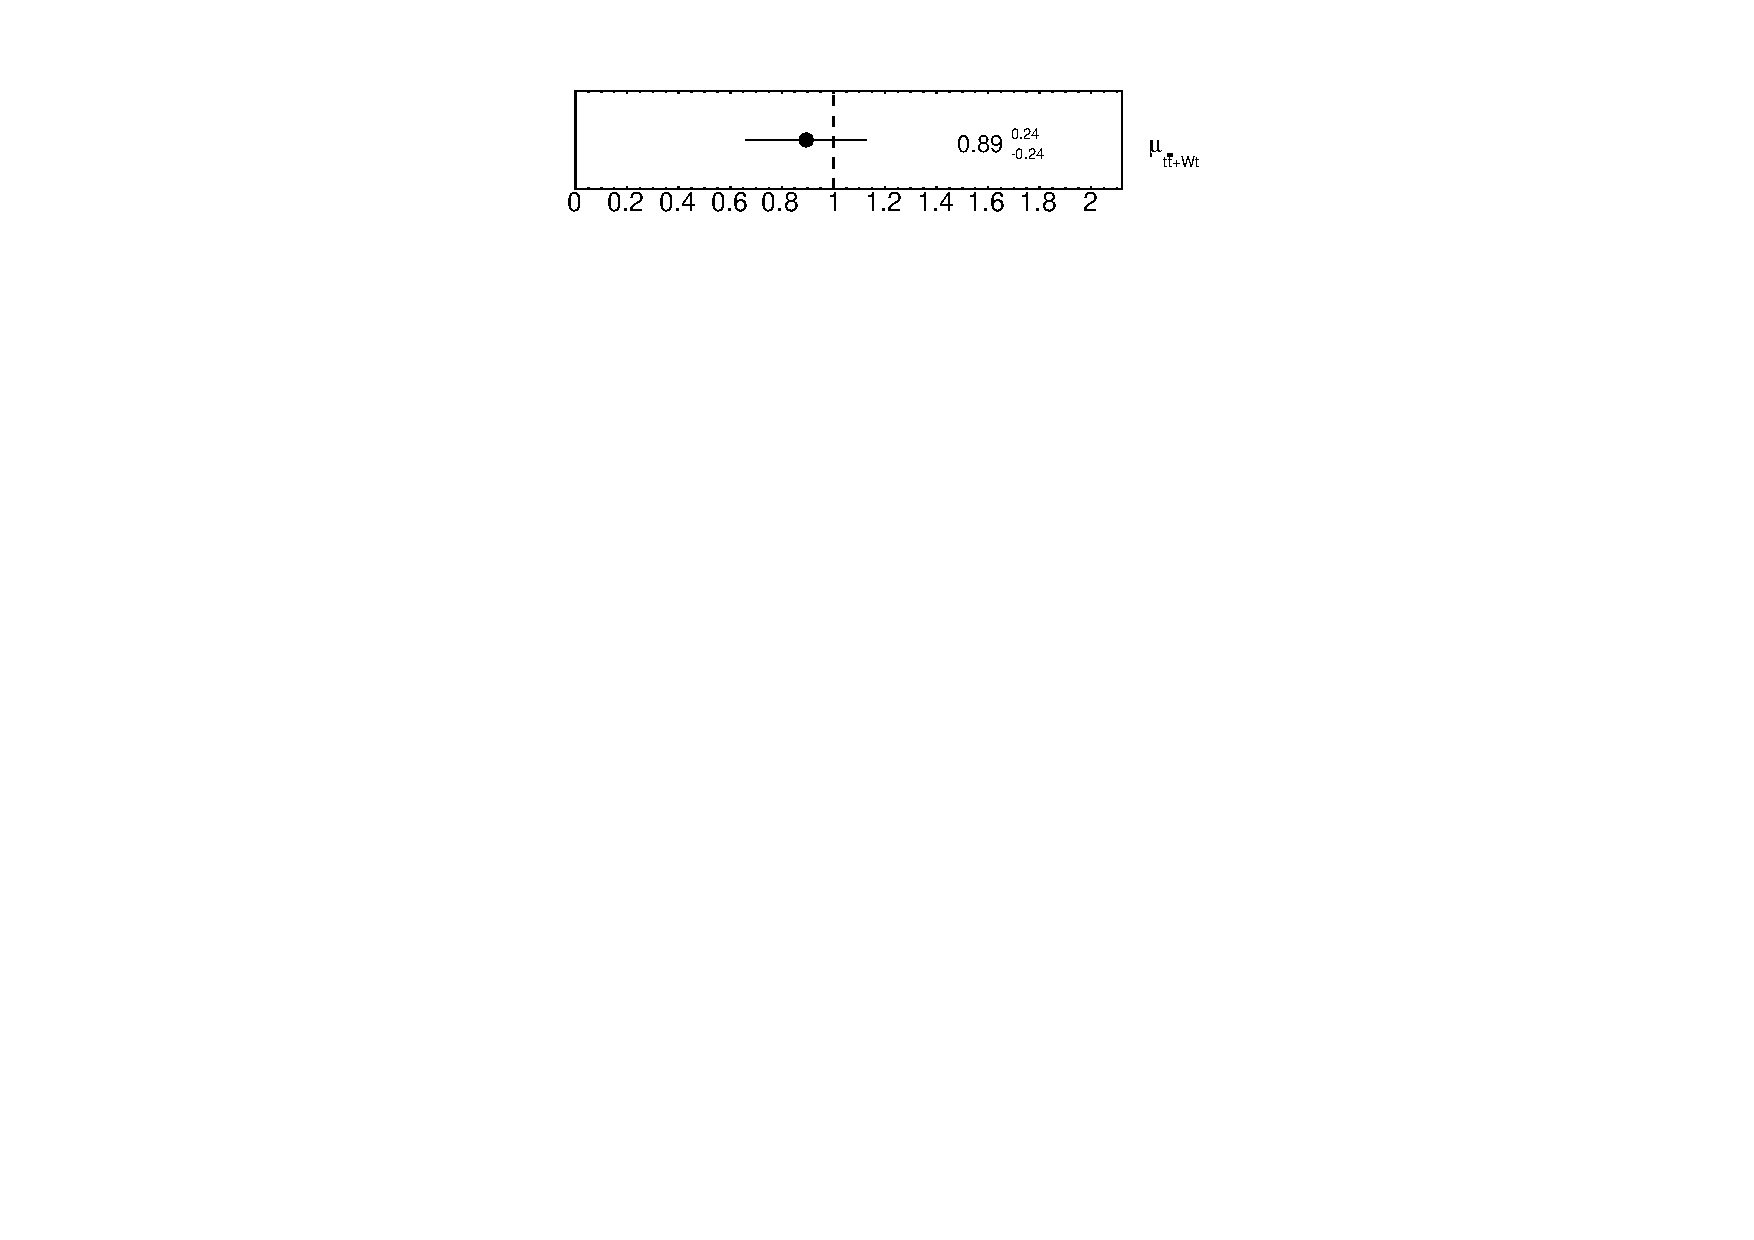
\includegraphics[width=.5\textwidth]{Appendices/AP9/figures/BONLY_CRSR_DL1rc_unblind/NormFactors}
	\caption{Normalisation factors for the B-only \tZc fit in SRs+CRs with data.}%
	\label{fig:stat:tzc:bonly:crsr:norm_unb}
\end{figure}
\restoregeometry

\begin{figure}[htbp]
	\centering
	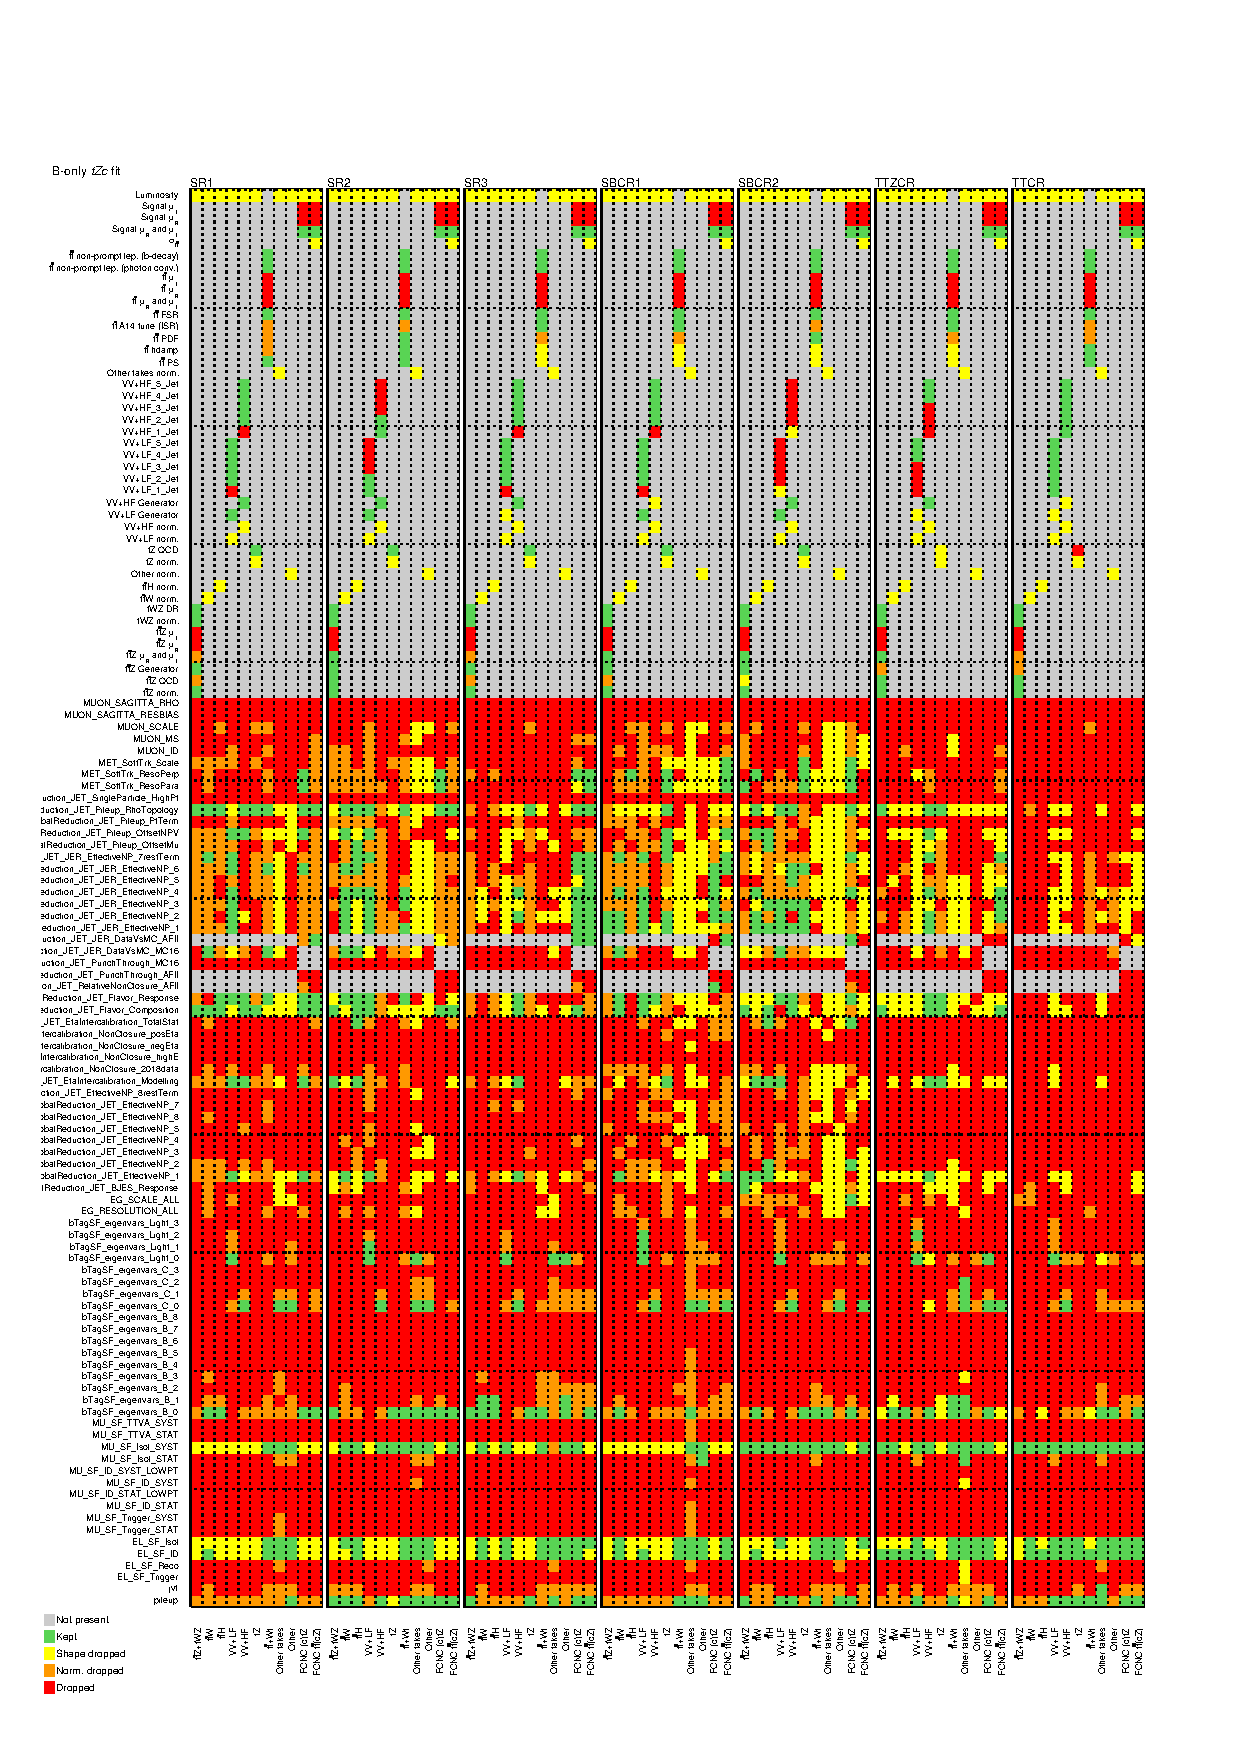
\includegraphics[width=.85\textwidth]{Appendices/AP9/figures/BONLY_CRSR_DL1rc_unblind/Pruning}
	\caption{Pruning of the nuisance parameters for the B-only fit in SRs+CRs with data.}%
	\label{fig:stat:tzc:bonly:crsr:pruning_unb}
\end{figure}

\begin{figure}[htbp]
	\centering
	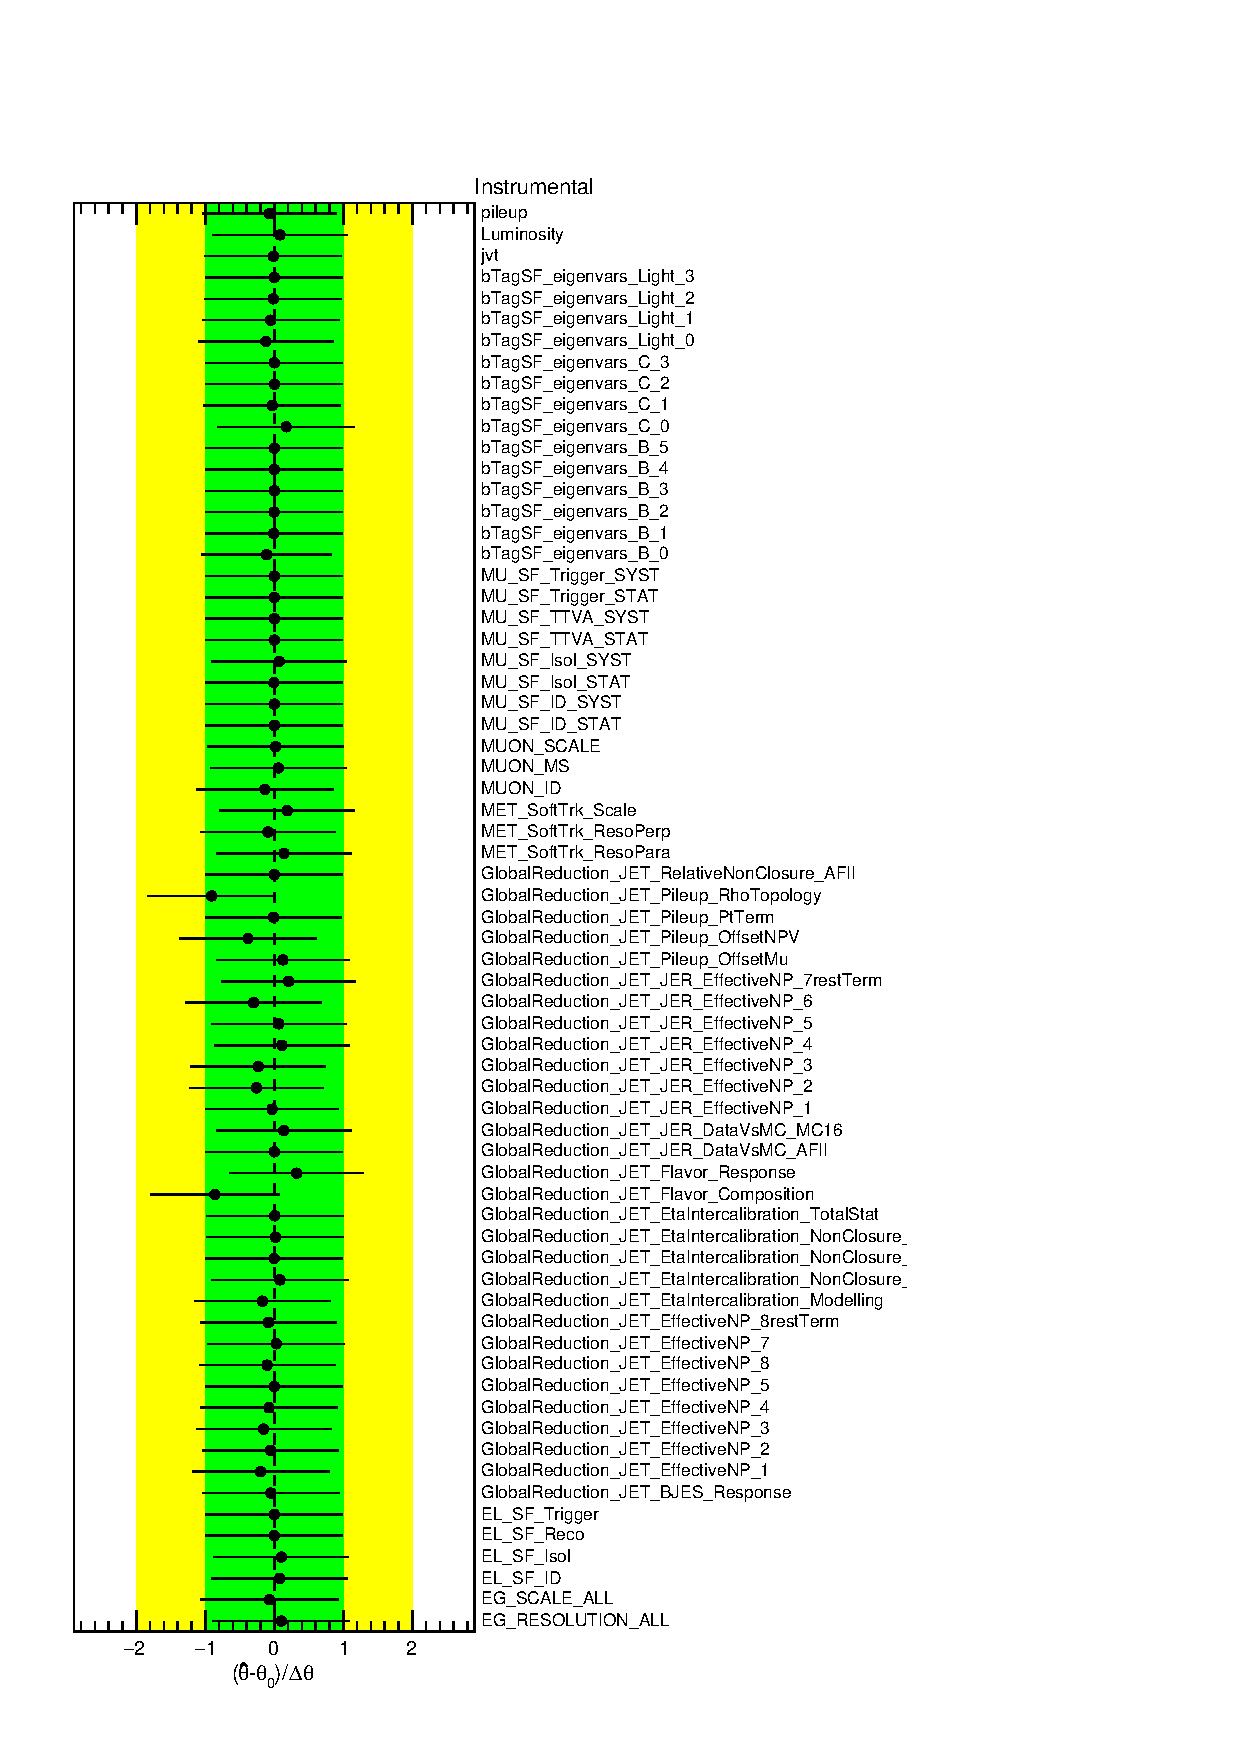
\includegraphics[width=.8\textwidth]{Appendices/AP9/figures/BONLY_CRSR_DL1rc_unblind/NuisPar_Instrumental}
	\caption{Pulls and constraints of the instrumental nuisance parameters for the B-only \tZc fit in SRs+CRs with data.}%
	\label{fig:stat:tzc:bonly:crsr:np:instr_unb}
\end{figure}

\begin{figure}[htbp]
	\centering
	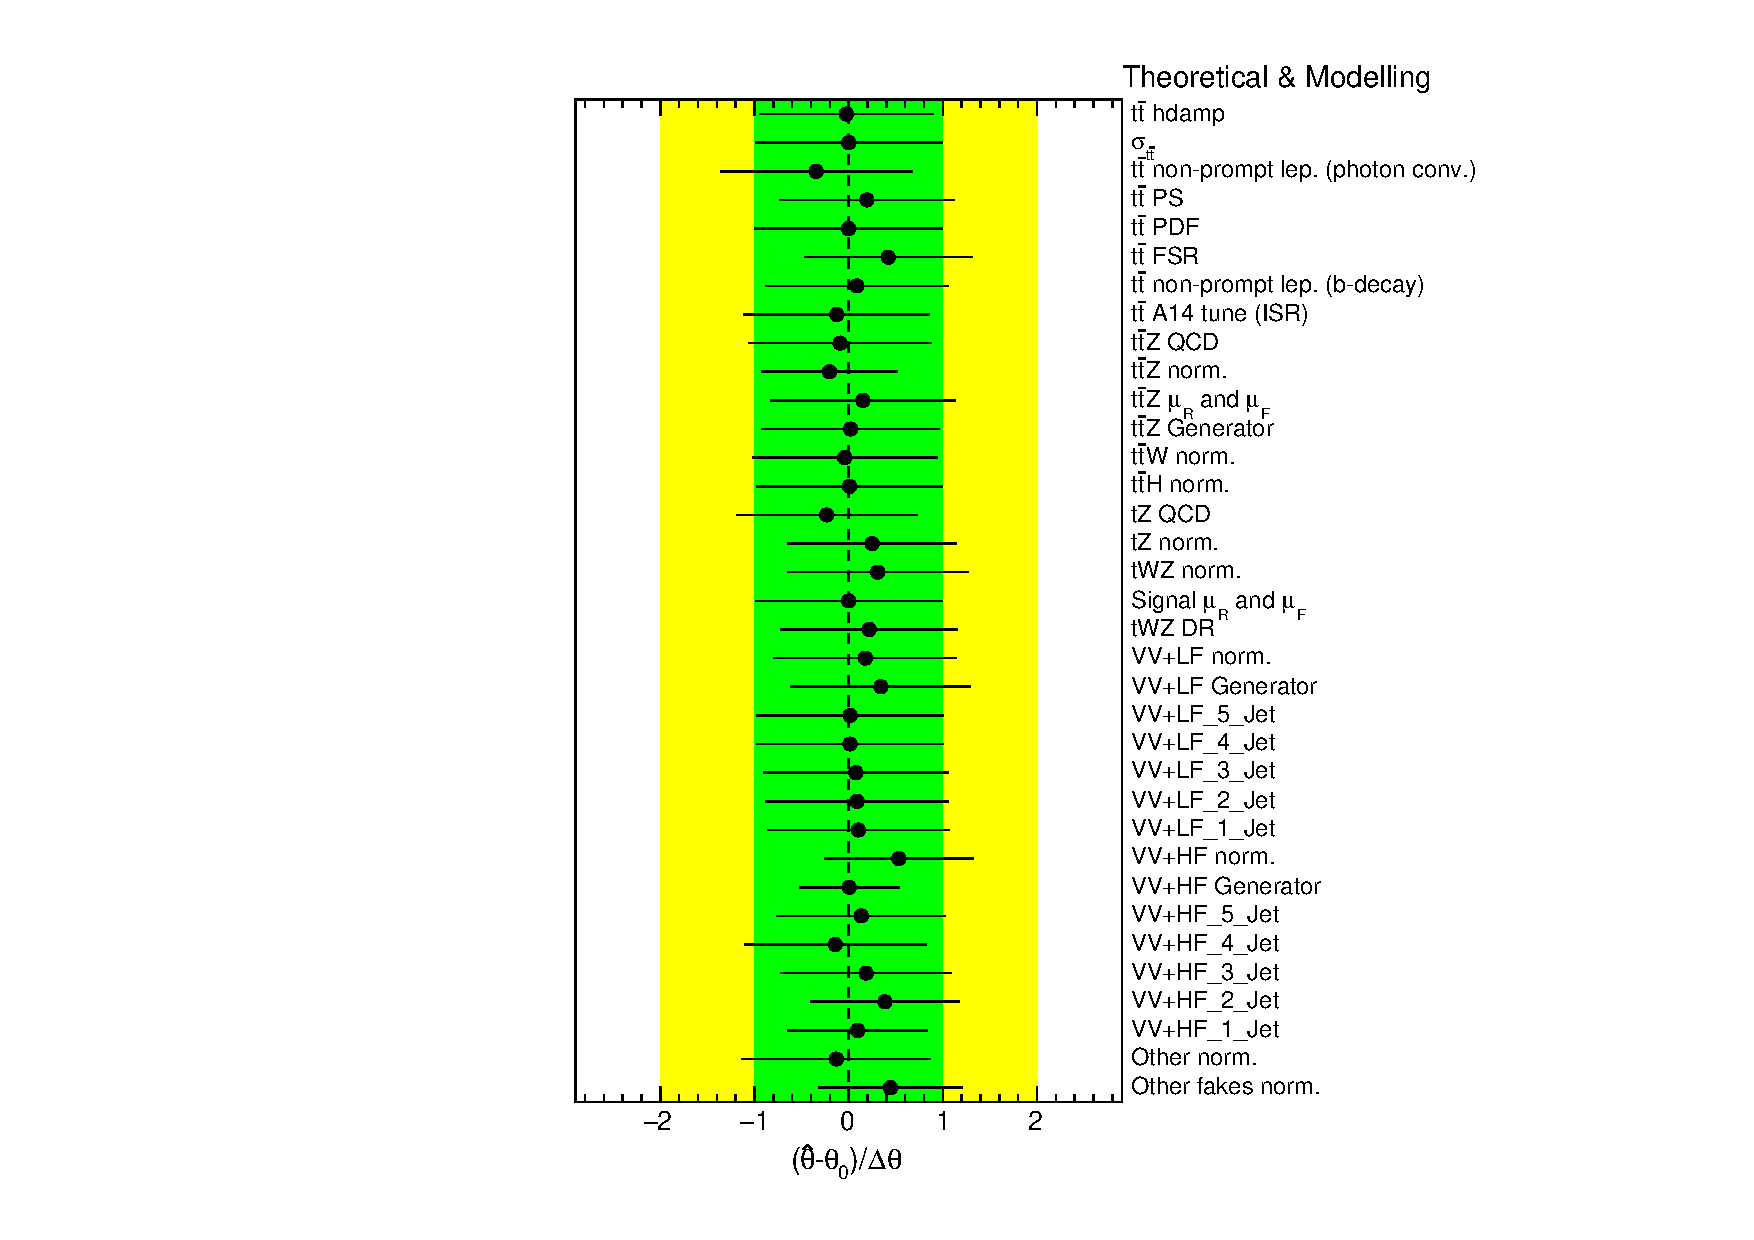
\includegraphics[width=.85\textwidth]{Appendices/AP9/figures/BONLY_CRSR_DL1rc_unblind/NuisPar_Theoretical_&_Modelling}
	\caption{Pulls and constraints of the theoretical and modeling nuisance parameters for the B-only \tZc fit in SRs+CRs with data.}%
	\label{fig:stat:tzc:bonly:crsr:np:model_unb}
\end{figure}

\begin{figure}[htbp]
	\centering
	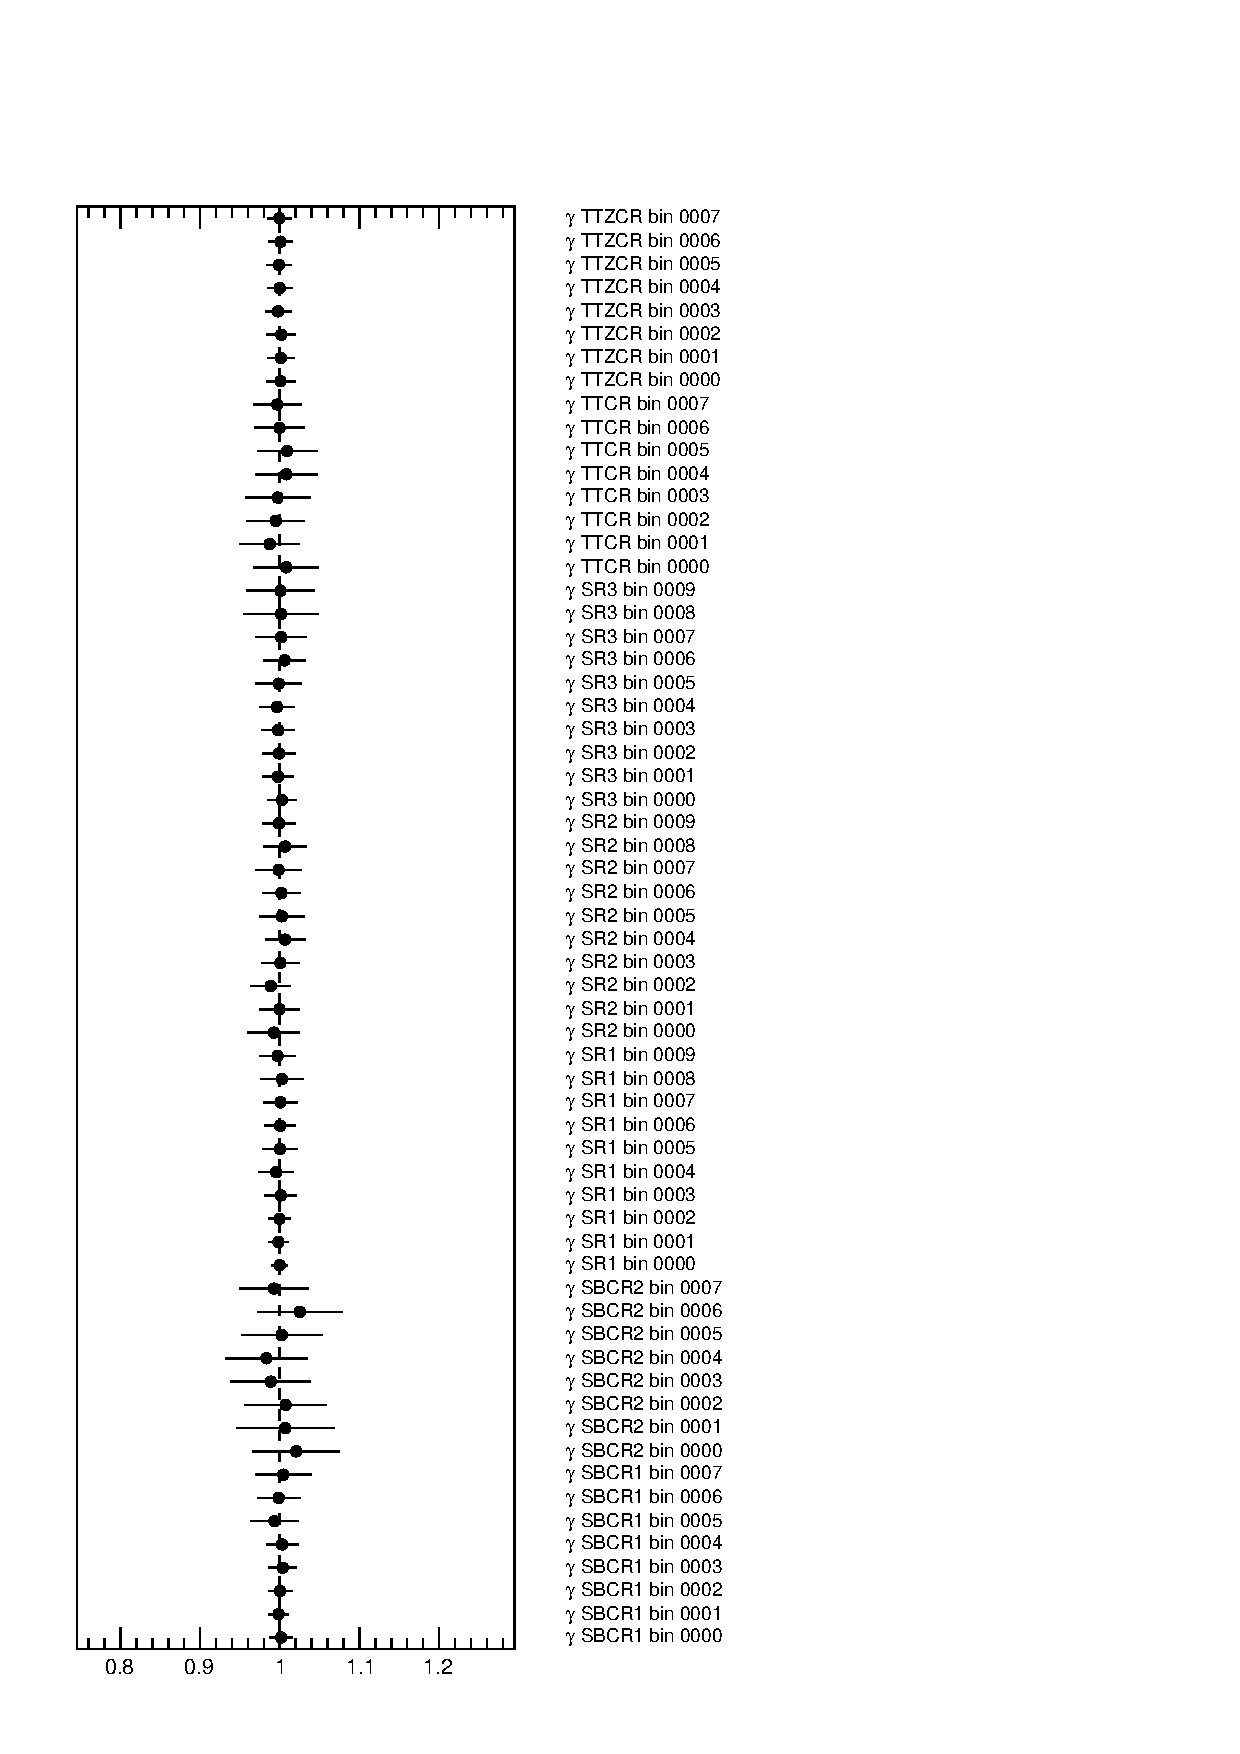
\includegraphics[width=.85\textwidth]{Appendices/AP9/figures/BONLY_CRSR_DL1rc_unblind/Gammas}
	\caption{Gamma parameters for the B-only \tZc fit in SRs+CRs with data.}%
	\label{fig:stat:tzc:bonly:crsr:gamma_unb}
\end{figure}

\begin{figure}[htbp]
	\centering
	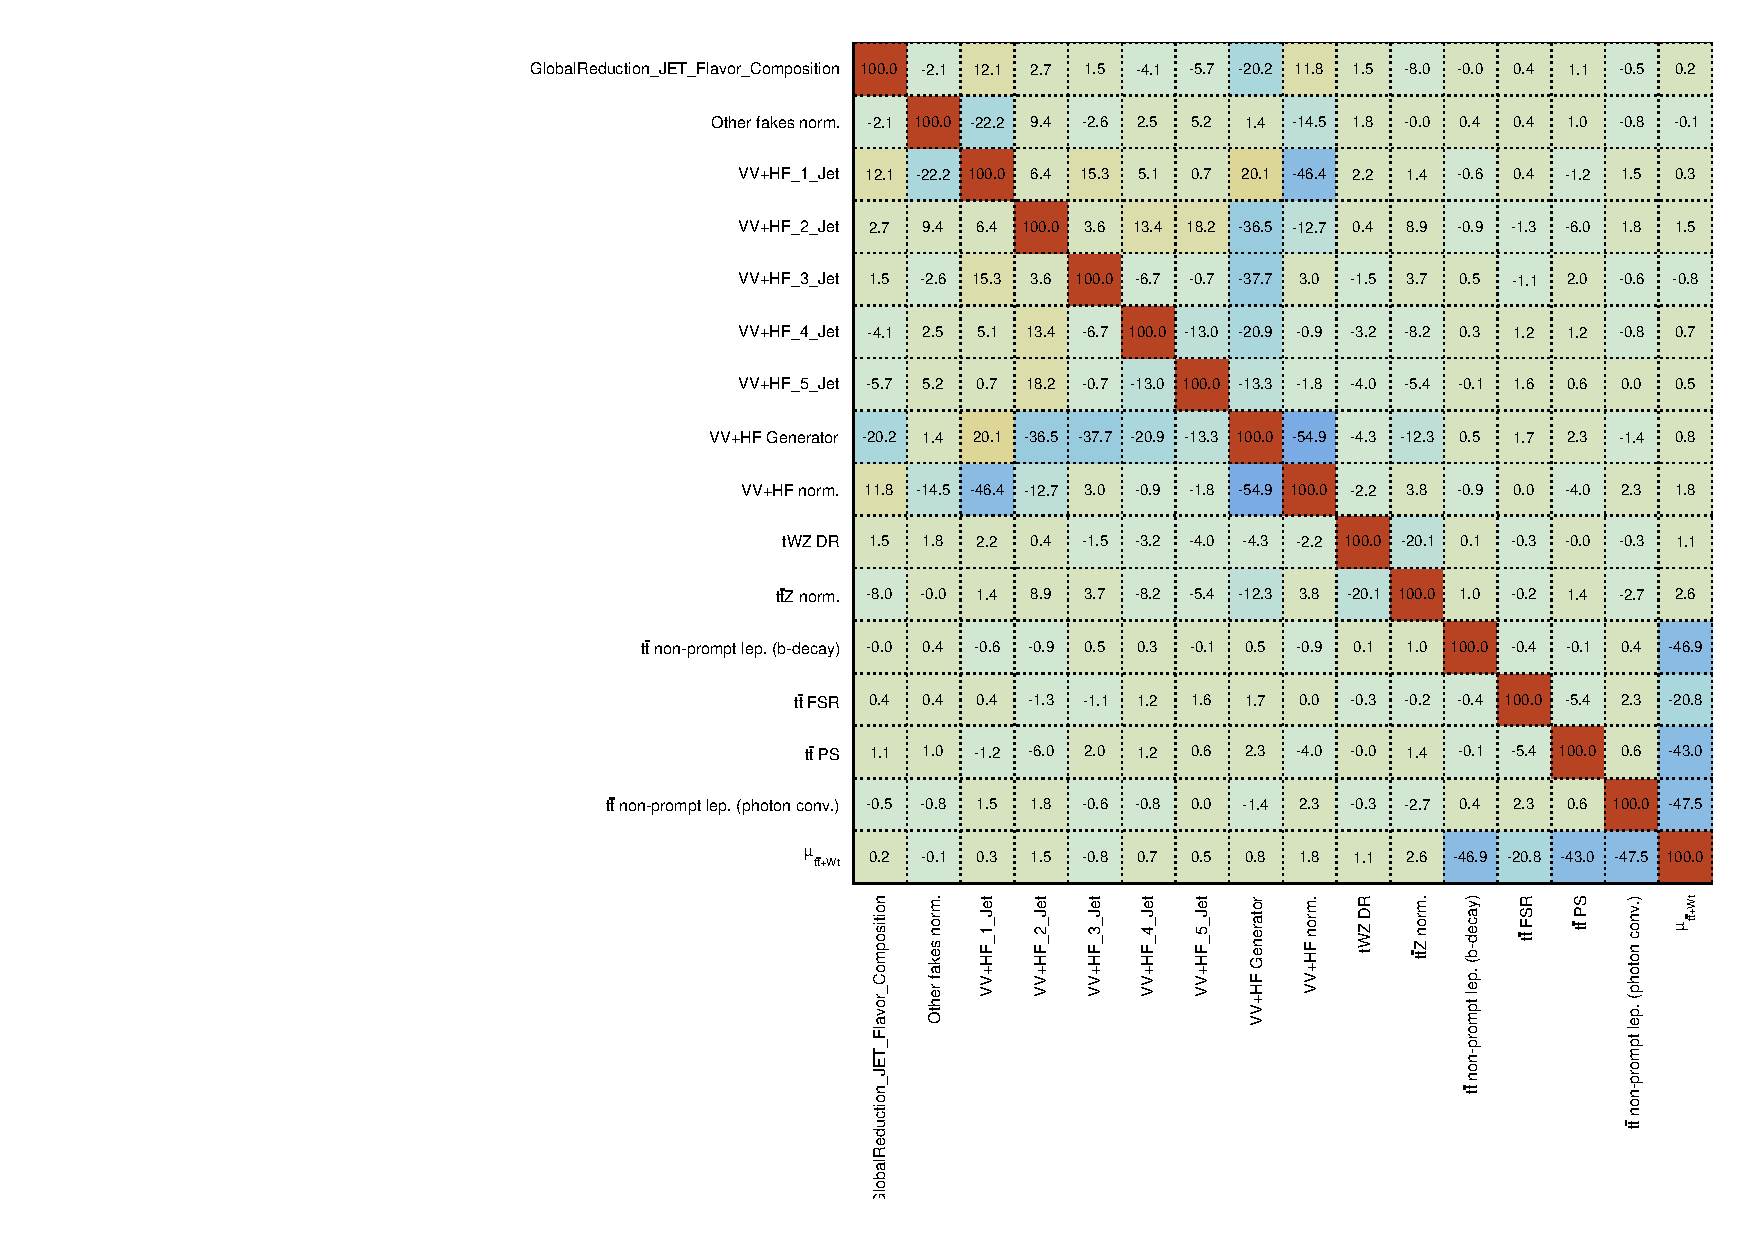
\includegraphics[width=.95\textwidth]{Appendices/AP9/figures/BONLY_CRSR_DL1rc_unblind/CorrMatrix}
	\caption{Correlation matrix of the nuisance paramenters for the B-only \tZc fit in SRs+CRs with data.}%
	\label{fig:stat:tzc:bonly:crsr:corrmatrix_unb}
\end{figure}

%\begin{figure}[htbp]
%	\centering
%	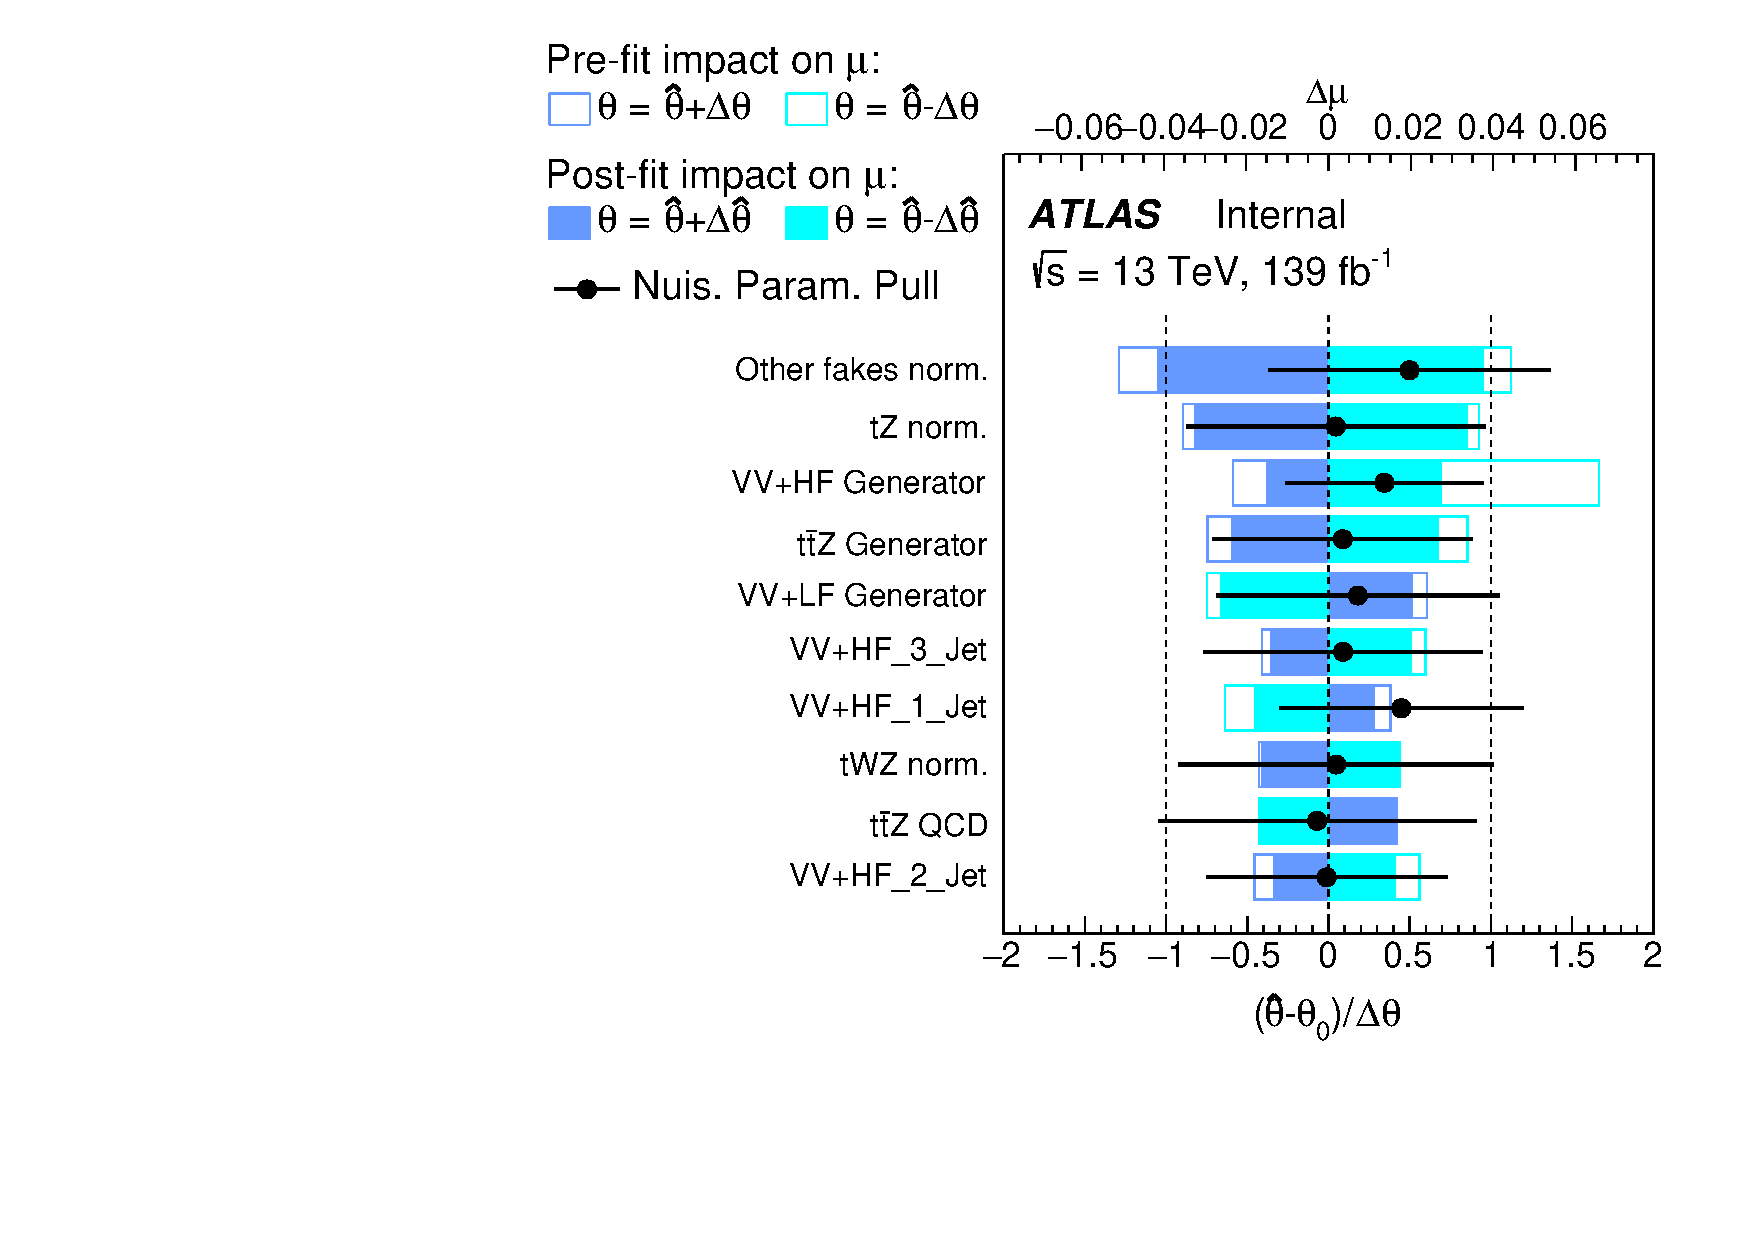
\includegraphics[width=.9\textwidth]{Appendices/AP9/figures/BONLY_CRSR_DL1rc_unblind/Ranking}
%	\caption{Ranking of the nuisance parameters for the B-only \tZc fit in SRs+CRs with data.}%
%	\label{fig:stat:tzc:bonly:crsr:ranking_unb}
%\end{figure}

\FloatBarrier
\clearpage
%\global\pdfpageattr\expandafter{\the\pdfpageattr/Rotate 90}
\begin{table}[]
	\centering
	\tiny
	% NB: add to main document: 
% \usepackage{siunitx} 
% \sisetup{separate-uncertainty,table-format=6.3(6)}  % hint: modify table-format to best fit your tables
\begin{tabular}{|p{0.10\textwidth}|>{\centering}p{0.08\textwidth}|>{\centering}p{0.08\textwidth}|>{\centering}p{0.08\textwidth}|>{\centering}p{0.09\textwidth}|>{\centering}p{0.09\textwidth}|>{\centering}p{0.09\textwidth}|>{\centering\arraybackslash}p{0.09\textwidth}|}
\toprule  
& {SR1} & {SR2} & {SR3} & {Side-band CR1} & {Side-band CR2} & {\ttZ CR} & {\ttbar CR}\\
\midrule 
    \ttZ+\tWZ   & 168 $\pm$ 22 & 33 $\pm$ 7 & 82 $\pm$ 11 & 88 $\pm$ 12 & 9.1 $\pm$ 2.1 & 164 $\pm$ 22 & 14.8 $\pm$ 1.9 \\ 
\ttW   & 5.8 $\pm$ 1.0 & 3.3 $\pm$ 0.6 & 2.04 $\pm$ 0.35 & 4.3 $\pm$ 0.7 & 2.5 $\pm$ 0.5 & 2.3 $\pm$ 0.5 & 27 $\pm$ 4 \\ 
\ttH   & 6.1 $\pm$ 1.0 & 0.88 $\pm$ 0.18 & 2.6 $\pm$ 0.4 & 2.3 $\pm$ 0.4 & 0.36 $\pm$ 0.07 & 5.4 $\pm$ 0.9 & 13.8 $\pm$ 2.1 \\ 
\VVLF   & 28 $\pm$ 17 & 35 $\pm$ 13 & 2.9 $\pm$ 2.0 & 25 $\pm$ 15 & 18 $\pm$ 7 & 0.20 $\pm$ 0.22 & 0.40 $\pm$ 0.21 \\ 
\VVHF   & 140 $\pm$ 100 & 160 $\pm$ 70 & 30 $\pm$ 22 & 130 $\pm$ 80 & 69 $\pm$ 28 & 13 $\pm$ 11 & 2.3 $\pm$ 1.4 \\ 
\tZq   & 47 $\pm$ 7 & 110 $\pm$ 18 & 13.8 $\pm$ 2.3 & 20 $\pm$ 4 & 9.9 $\pm$ 1.7 & 14.6 $\pm$ 2.9 & 0.90 $\pm$ 0.15 \\ 
\ttbar+Wt   & 21 $\pm$ 4 & 32 $\pm$ 11 & 3.7 $\pm$ 1.0 & 10 $\pm$ 4 & 9.1 $\pm$ 2.7 & 3.0 $\pm$ 1.2 & 102 $\pm$ 24 \\ 
Other fakes   & 10 $\pm$ 11 & 12 $\pm$ 12 & 1.4 $\pm$ 1.6 & 3 $\pm$ 5 & 10 $\pm$ 11 & 0.00 $\pm$ 0.06 & 0.12 $\pm$ 0.14 \\ 
Other   & 2.5 $\pm$ 1.5 & 3.8 $\pm$ 2.8 & 0.48 $\pm$ 0.25 & 2.2 $\pm$ 1.6 & 0.8 $\pm$ 2.6 & 1.1 $\pm$ 0.5 & 2.9 $\pm$ 1.5 \\ 
\midrule 
Total background  & 430 $\pm$ 110 & 390 $\pm$ 80 & 139 $\pm$ 25 & 280 $\pm$ 80 & 130 $\pm$ 32 & 203 $\pm$ 27 & 164 $\pm$ 25 \\ 
\midrule 
Data   & 433 & 443 & 143 & 331 & 169 & 197 & 156 \\ 
\midrule 
Data / Bkg.   & 1.00 $\pm$ 0.25 & 1.15 $\pm$ 0.24 & 1.03 $\pm$ 0.20 & 1.18 $\pm$ 0.35 & 1.30 $\pm$ 0.34 & 0.97 $\pm$ 0.14 & 0.95 $\pm$ 0.16 \\ 
\bottomrule 
\end{tabular} 

	\caption{Pre-fit event yields in the B-only \tZc fit in SRs+CRs with data. \TabErrStatSys} 
	\label{tab:stat:tzc:bonly:crsr:yields:prefit_unb}
\end{table} 

\begin{table}[]
	\centering
	\tiny
	% NB: add to main document: 
% \usepackage{siunitx} 
% \sisetup{separate-uncertainty,table-format=6.3(6)}  % hint: modify table-format to best fit your tables
\begin{tabular}{|p{0.10\textwidth}|>{\centering}p{0.08\textwidth}|>{\centering}p{0.08\textwidth}|>{\centering}p{0.08\textwidth}|>{\centering}p{0.09\textwidth}|>{\centering}p{0.09\textwidth}|>{\centering}p{0.09\textwidth}|>{\centering\arraybackslash}p{0.09\textwidth}|}
\toprule  
 & {SR1} & {SR2} & {SR3} & {Side-band CR1} & {Side-band CR2} & {\ttZ CR} & {\ttbar CR}\\
\midrule 
   \ttZ+\tWZ   & 166 $\pm$ 14 & 39 $\pm$ 7 & 82 $\pm$ 7 & 90 $\pm$ 9 & 10.5 $\pm$ 2.1 & 156 $\pm$ 13 & 15.0 $\pm$ 1.4 \\ 
\ttW   & 5.6 $\pm$ 0.9 & 3.6 $\pm$ 0.6 & 2.03 $\pm$ 0.32 & 4.0 $\pm$ 0.6 & 2.7 $\pm$ 0.5 & 2.0 $\pm$ 0.4 & 27 $\pm$ 4 \\ 
\ttH   & 5.9 $\pm$ 0.9 & 1.02 $\pm$ 0.20 & 2.6 $\pm$ 0.4 & 2.3 $\pm$ 0.4 & 0.42 $\pm$ 0.08 & 5.1 $\pm$ 0.8 & 14.0 $\pm$ 2.1 \\ 
\VVLF   & 31 $\pm$ 18 & 37 $\pm$ 13 & 3.3 $\pm$ 2.1 & 30 $\pm$ 17 & 21 $\pm$ 8 & 0.20 $\pm$ 0.19 & 0.36 $\pm$ 0.17 \\ 
\VVHF   & 162 $\pm$ 28 & 192 $\pm$ 29 & 35 $\pm$ 6 & 152 $\pm$ 24 & 85 $\pm$ 16 & 13 $\pm$ 5 & 2.7 $\pm$ 0.5 \\ 
\tZq   & 47 $\pm$ 6 & 120 $\pm$ 17 & 14.4 $\pm$ 2.1 & 20.2 $\pm$ 3.4 & 10.8 $\pm$ 1.6 & 14.2 $\pm$ 2.4 & 0.95 $\pm$ 0.12 \\ 
\ttbar+Wt   & 16.9 $\pm$ 3.1 & 32 $\pm$ 7 & 3.0 $\pm$ 0.6 & 10.0 $\pm$ 3.0 & 9.0 $\pm$ 1.7 & 2.2 $\pm$ 0.7 & 94 $\pm$ 13 \\ 
Other fakes   & 13 $\pm$ 8 & 16 $\pm$ 10 & 2.0 $\pm$ 1.4 & 4 $\pm$ 4 & 23 $\pm$ 16 & 0.005 $\pm$ 0.008 & 0.17 $\pm$ 0.11 \\ 
Other   & 1.9 $\pm$ 1.0 & 3.3 $\pm$ 2.2 & 0.44 $\pm$ 0.23 & 1.8 $\pm$ 1.2 & 0.3 $\pm$ 1.2 & 1.0 $\pm$ 0.5 & 2.7 $\pm$ 1.4 \\ 
\midrule 
Total background  & 449 $\pm$ 17 & 444 $\pm$ 19 & 144 $\pm$ 6 & 315 $\pm$ 16 & 163 $\pm$ 13 & 194 $\pm$ 12 & 156 $\pm$ 12 \\ 
\midrule 
Data   & 433 & 443 & 143 & 331 & 169 & 197 & 156 \\ 
\midrule 
Data / Bkg.   & 0.96 $\pm$ 0.04 & 1.00 $\pm$ 0.04 & 0.99 $\pm$ 0.04 & 1.05 $\pm$ 0.05 & 1.04 $\pm$ 0.09 & 1.02 $\pm$ 0.06 & 1.00 $\pm$ 0.08 \\ 
\bottomrule 
\end{tabular} 

	\caption{Post-fit event yields in the B-only\tZc fit in SRs+CRs with data. \TabErrStatSys} 
	\label{tab:stat:tzc:bonly:crsr:yields:postfit_unb}
\end{table} 
\clearpage
\FloatBarrier
%\global\pdfpageattr\expandafter{\the\pdfpageattr/Rotate 0}

\clearpage
\begin{figure}[htbp]
	\centering
	\begin{tabular}{cc}
		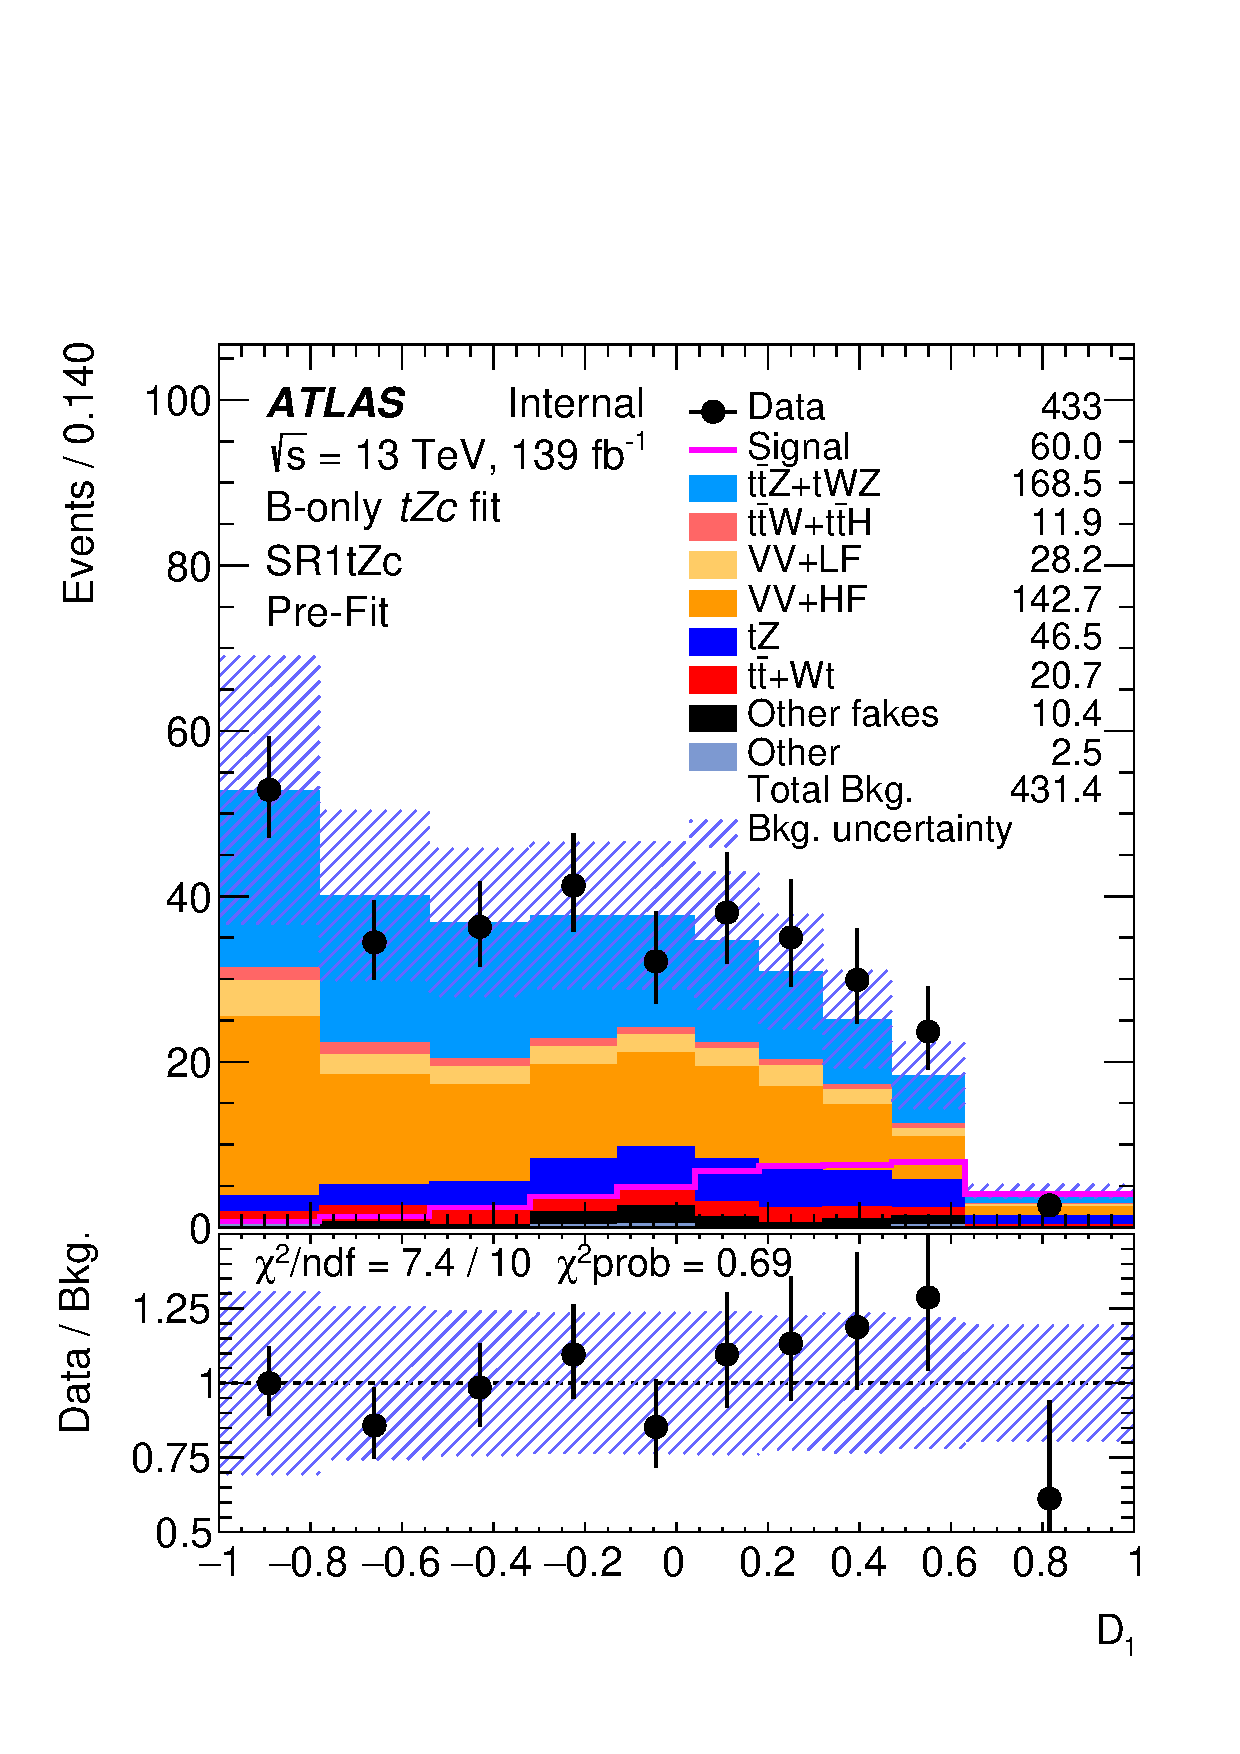
\includegraphics[width=.45\textwidth]{Appendices/AP9/figures/BONLY_CRSR_DL1rc_unblind/Plots/SR1} &
		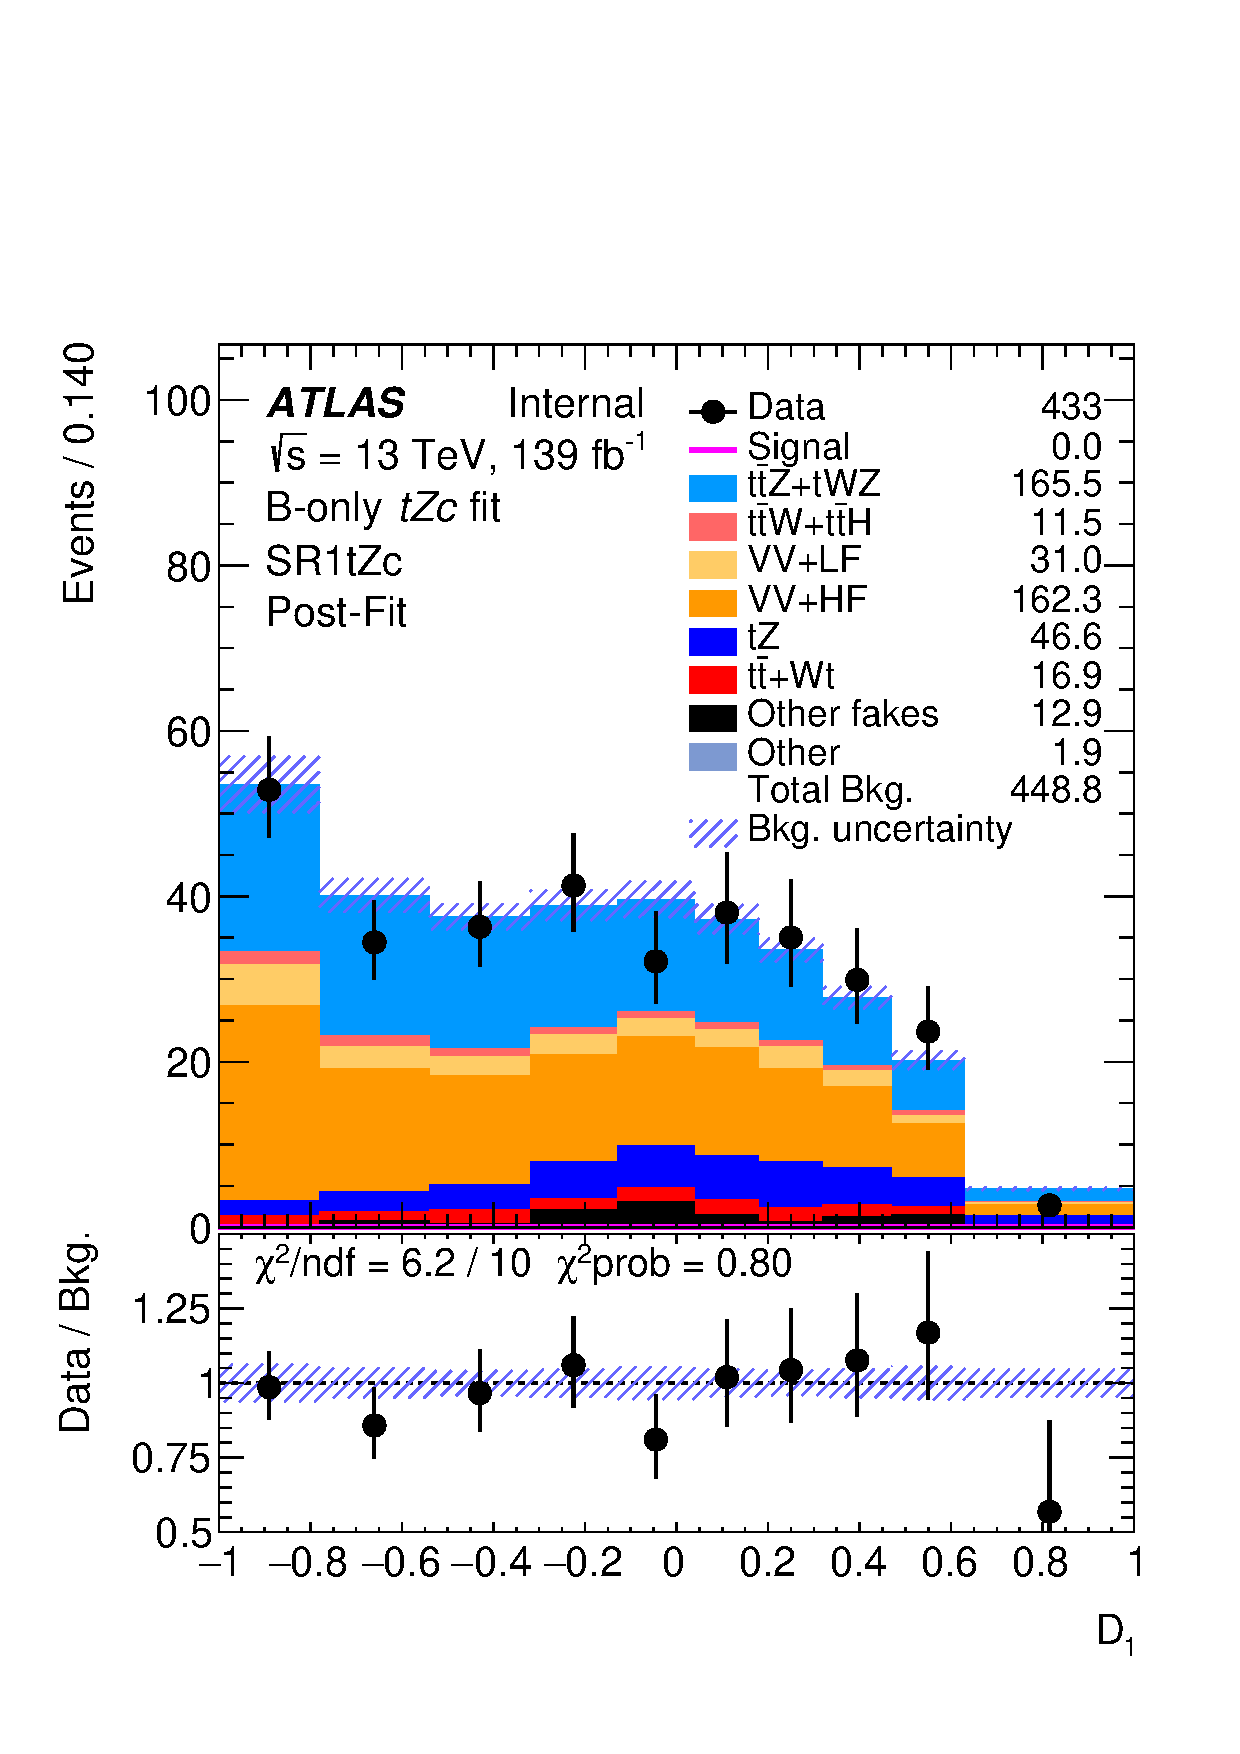
\includegraphics[width=.45\textwidth]{Appendices/AP9/figures/BONLY_CRSR_DL1rc_unblind/Plots/SR1_postFit} \\
		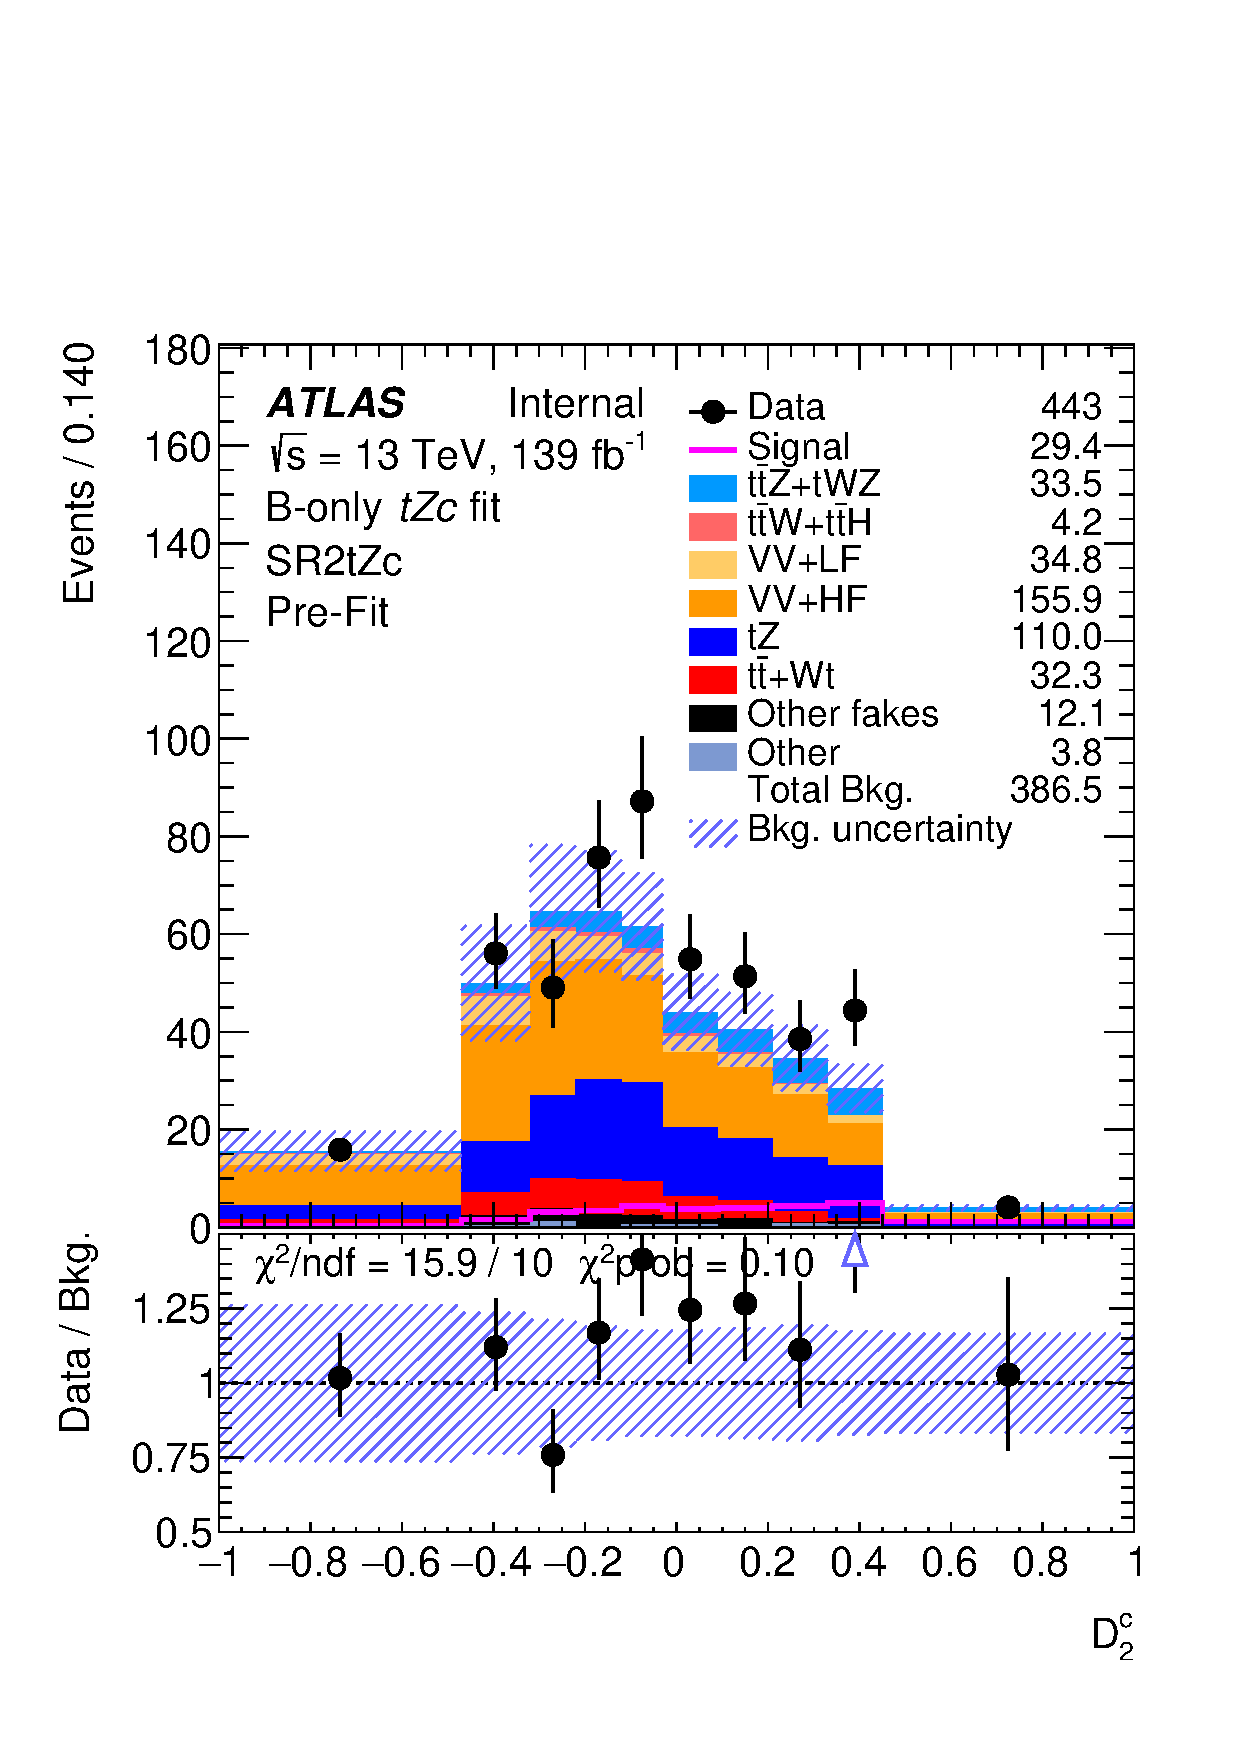
\includegraphics[width=.45\textwidth]{Appendices/AP9/figures/BONLY_CRSR_DL1rc_unblind/Plots/SR2} &
		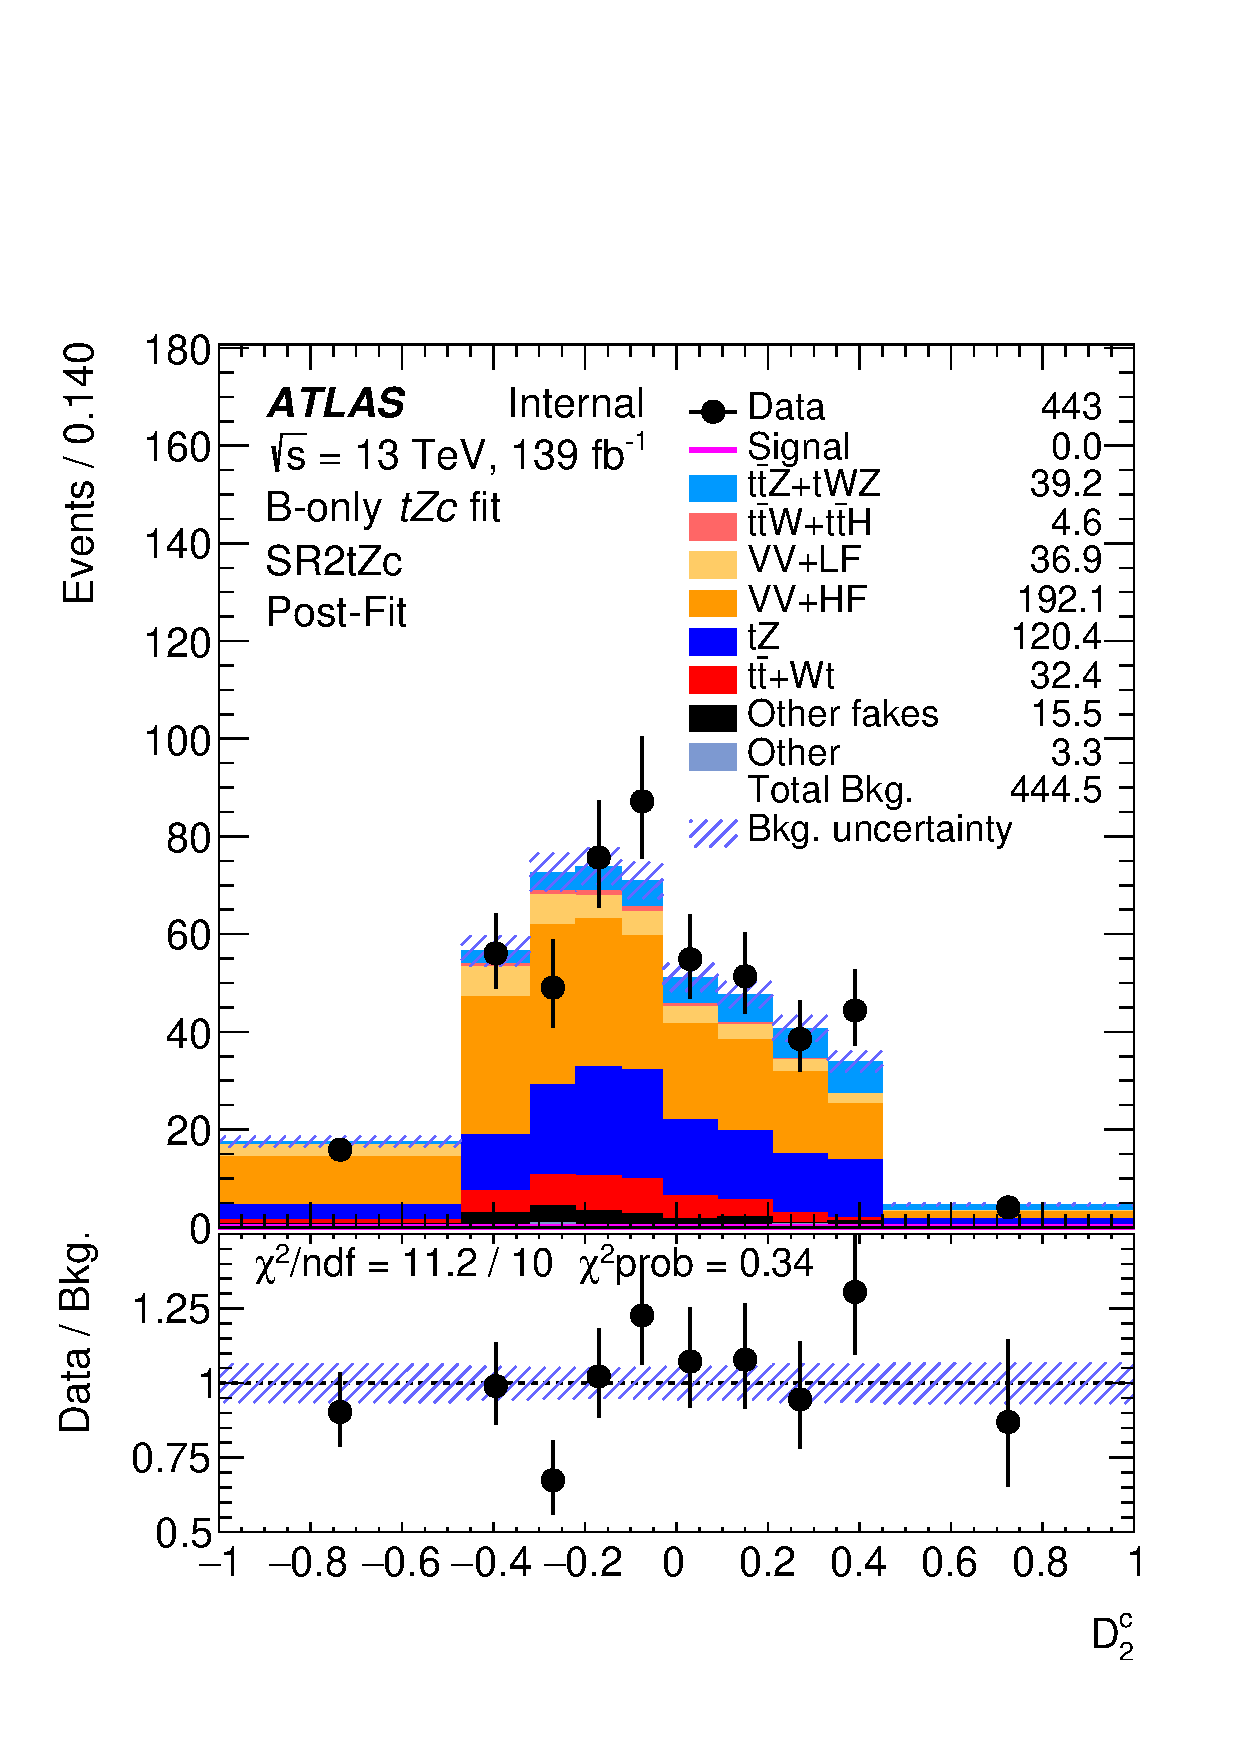
\includegraphics[width=.45\textwidth]{Appendices/AP9/figures/BONLY_CRSR_DL1rc_unblind/Plots/SR2_postFit} \\
	\end{tabular}
	\caption{Pre-fit (left) and post-fit (right) BDTG output distributions in SR1 and SR2 for the B-only \tZc fit in SRs+CRs with data.
		\ErrStatSys
	}%
	\label{fig:stat:tzc:bonly:crsr:srplots:1_unb}
\end{figure}

\begin{figure}[htbp]
	\centering
	\begin{tabular}{cc}
		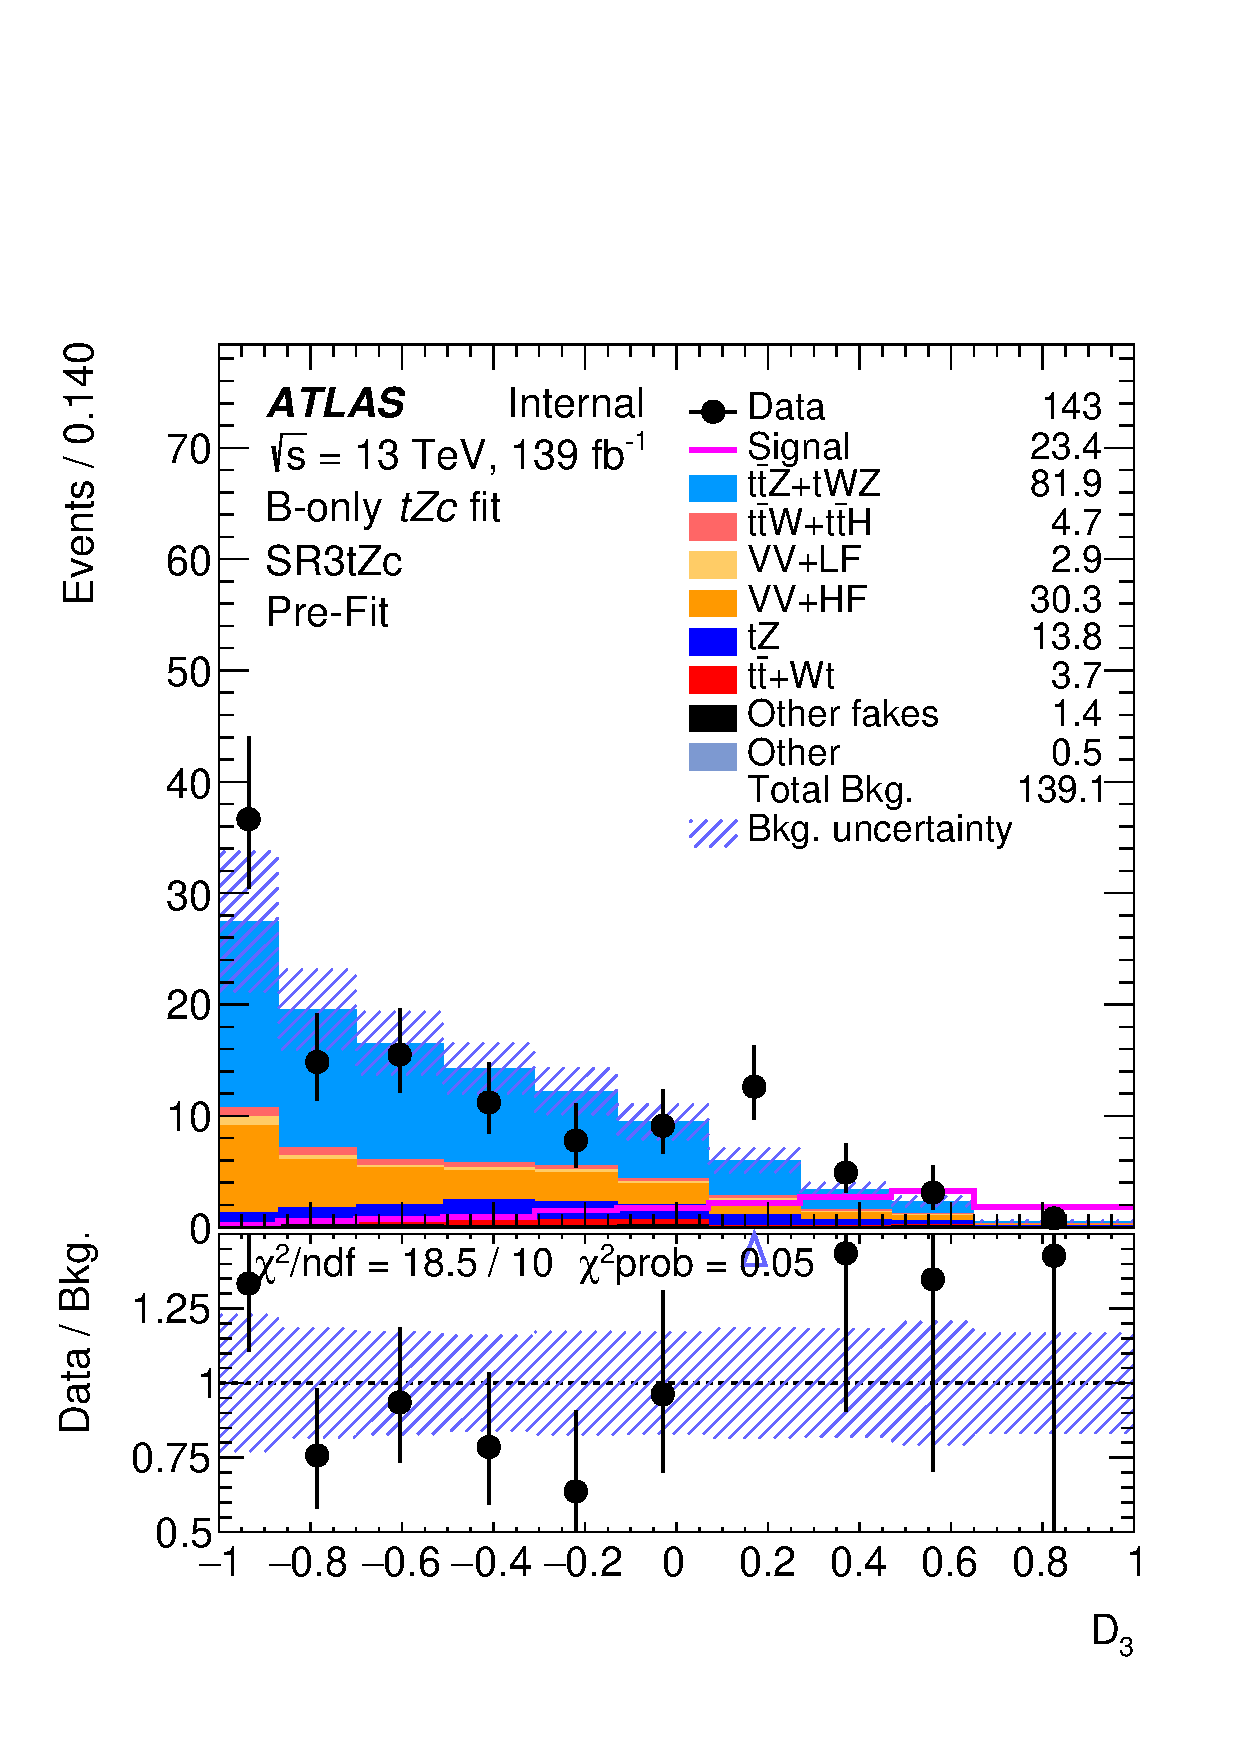
\includegraphics[width=.45\textwidth]{Appendices/AP9/figures/BONLY_CRSR_DL1rc_unblind/Plots/SR3} &
		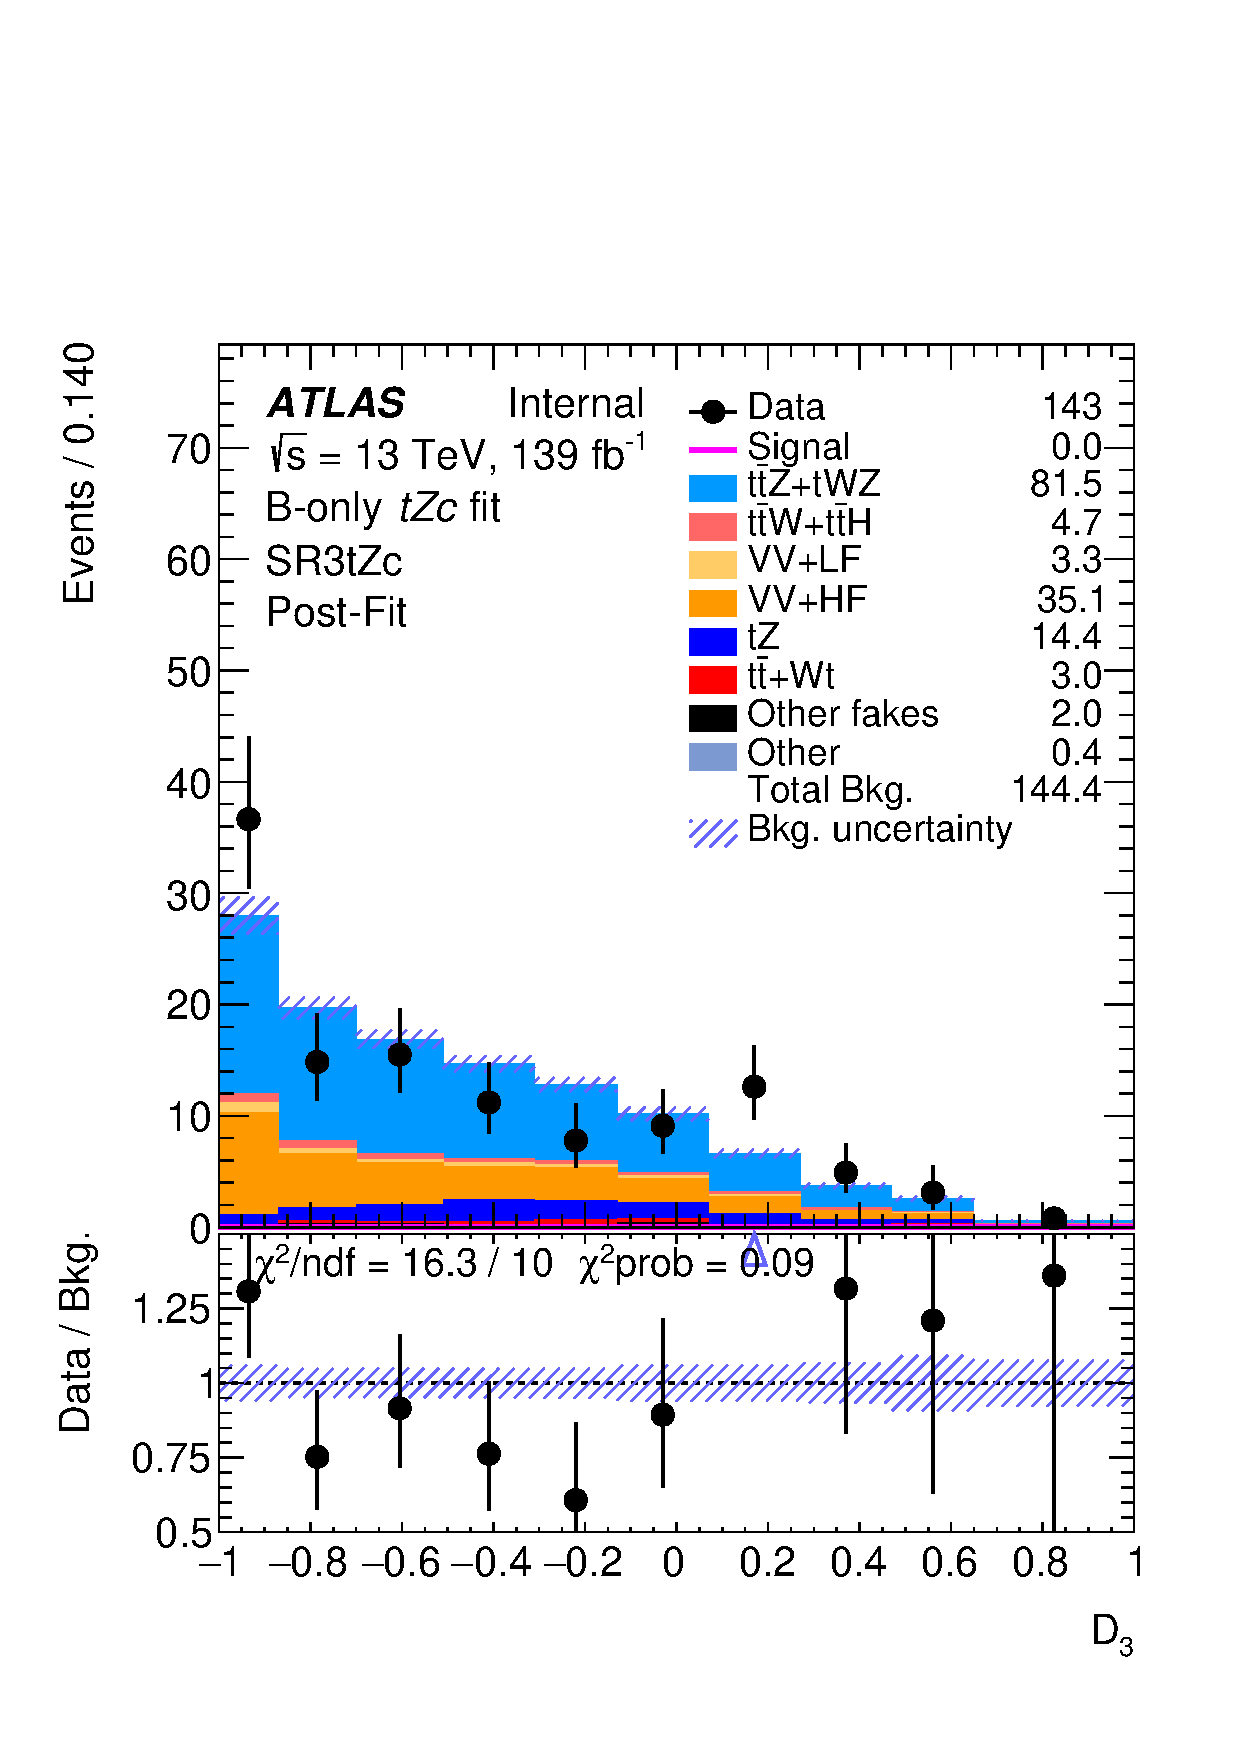
\includegraphics[width=.45\textwidth]{Appendices/AP9/figures/BONLY_CRSR_DL1rc_unblind/Plots/SR3_postFit} \\
	\end{tabular}
	\caption{Pre-fit (left) and post-fit (right) leading lepton \pt distributions in SR3 for the B-only \tZc fit in SRs+CRs with data.
		\ErrStatSys
	}%
	\label{fig:stat:tzc:bonly:crsr:srplots:2_unb}
\end{figure}

\begin{figure}[htbp]
	\centering
	\begin{tabular}{cc}
		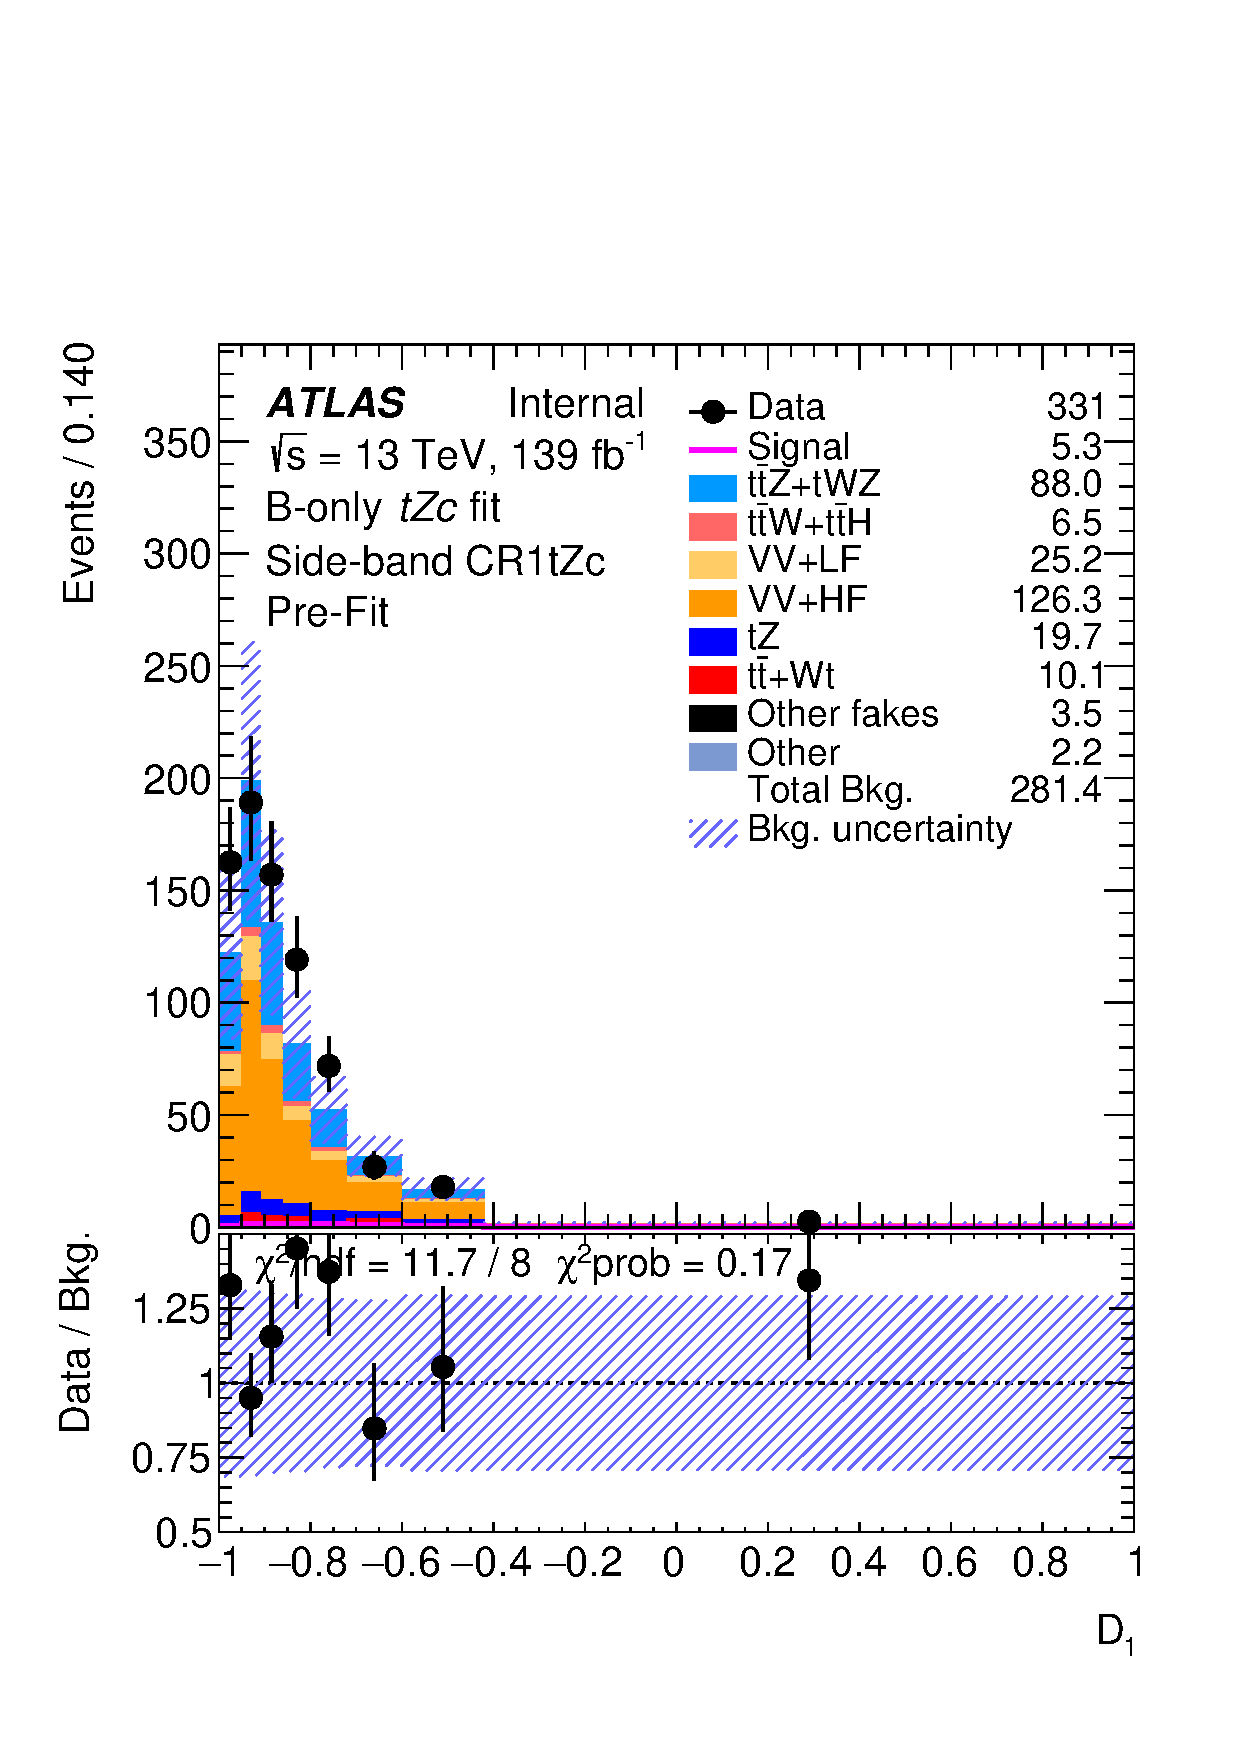
\includegraphics[width=.45\textwidth]{Appendices/AP9/figures/BONLY_CRSR_DL1rc_unblind/Plots/SBCR1} &
		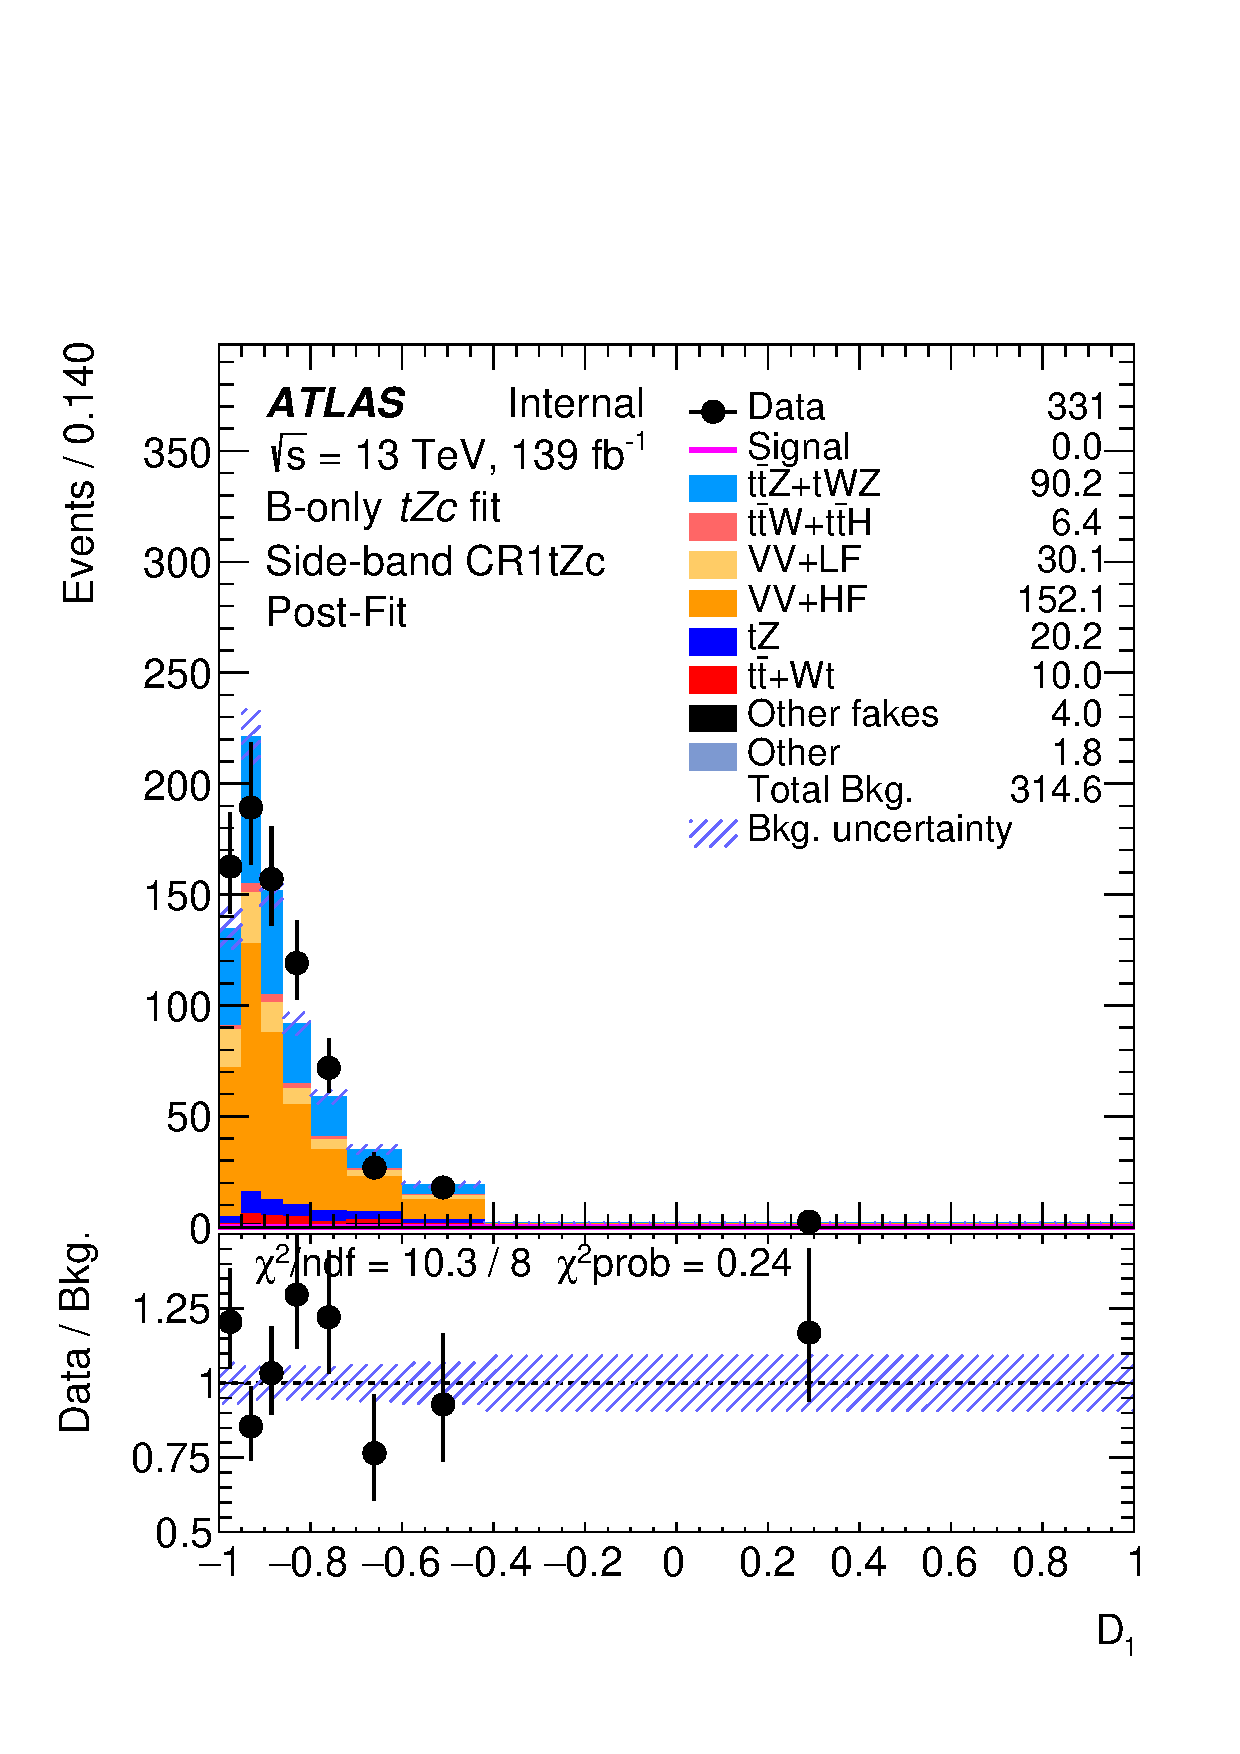
\includegraphics[width=.45\textwidth]{Appendices/AP9/figures/BONLY_CRSR_DL1rc_unblind/Plots/SBCR1_postFit} \\
		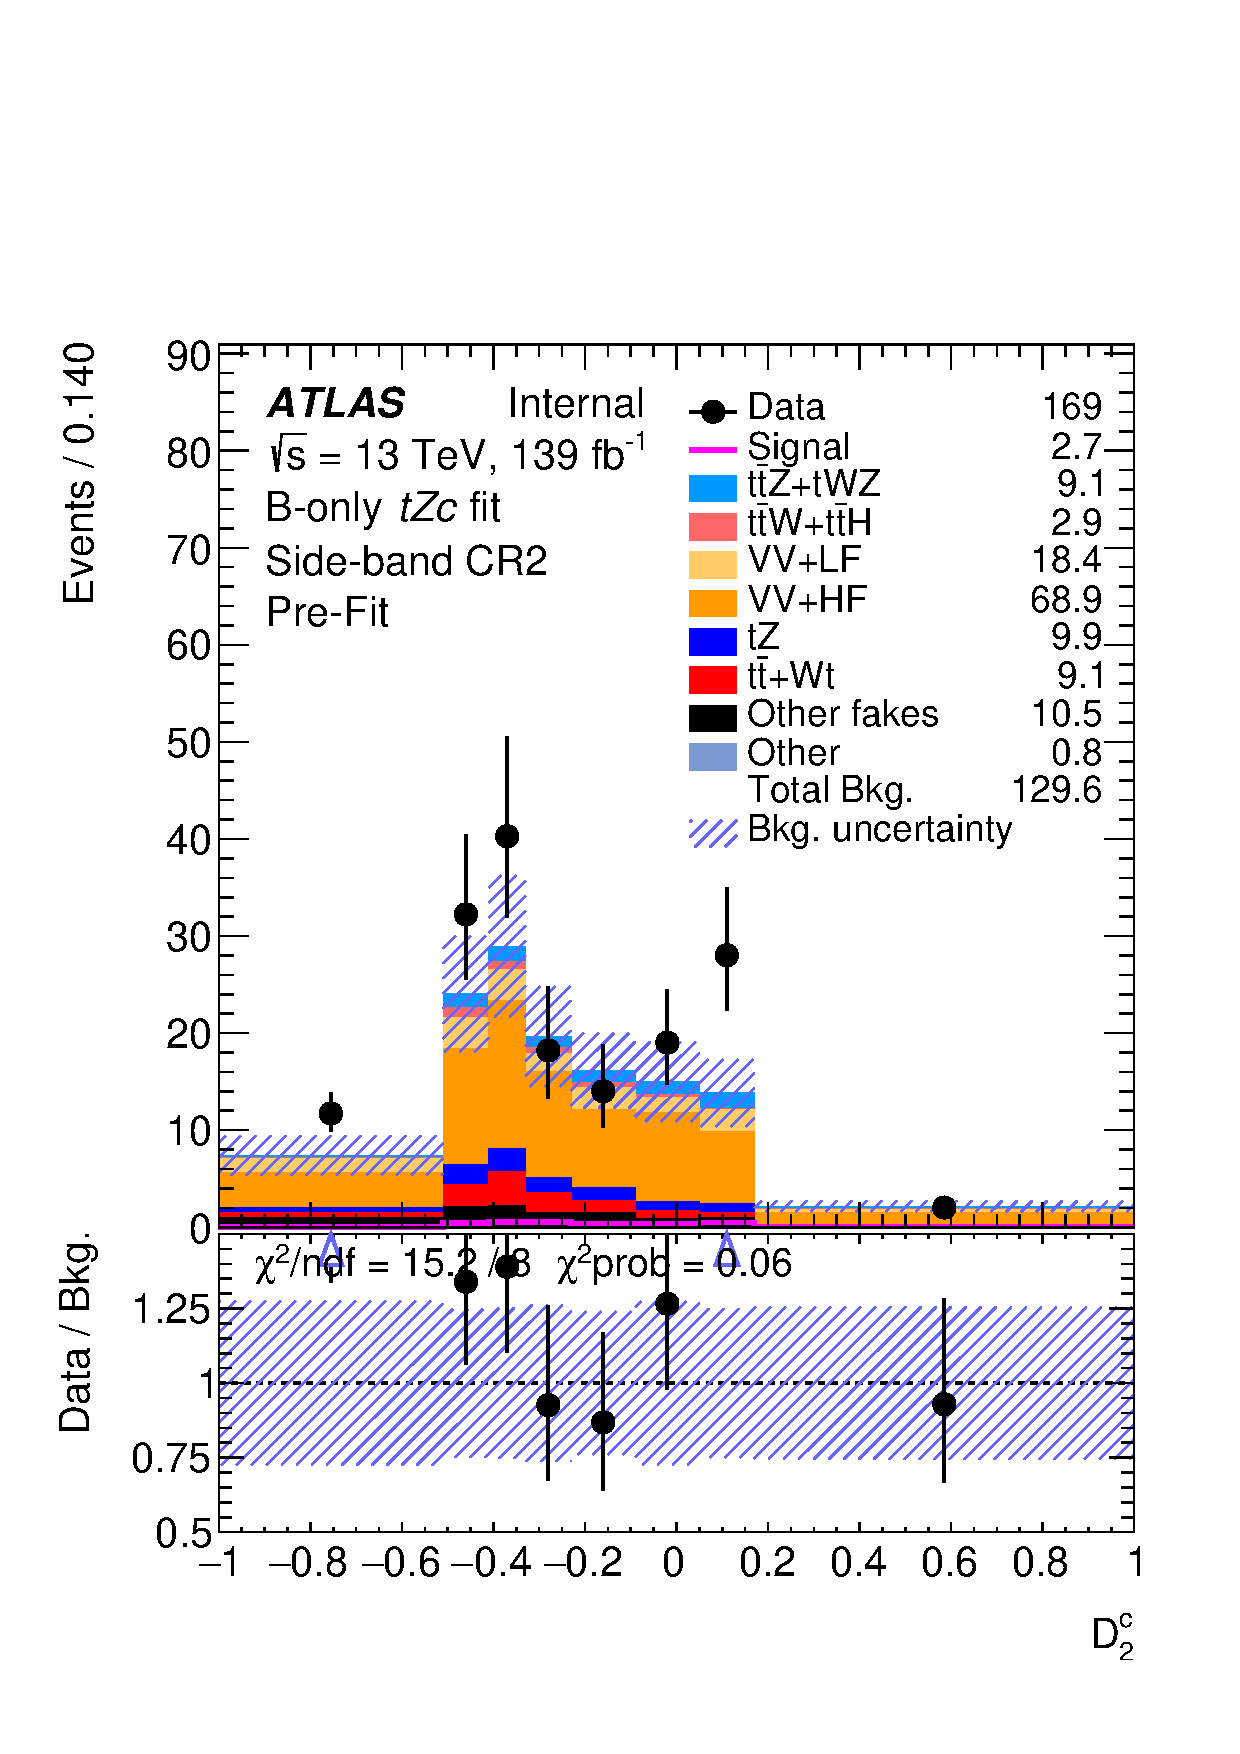
\includegraphics[width=.45\textwidth]{Appendices/AP9/figures/BONLY_CRSR_DL1rc_unblind/Plots/SBCR2} &
		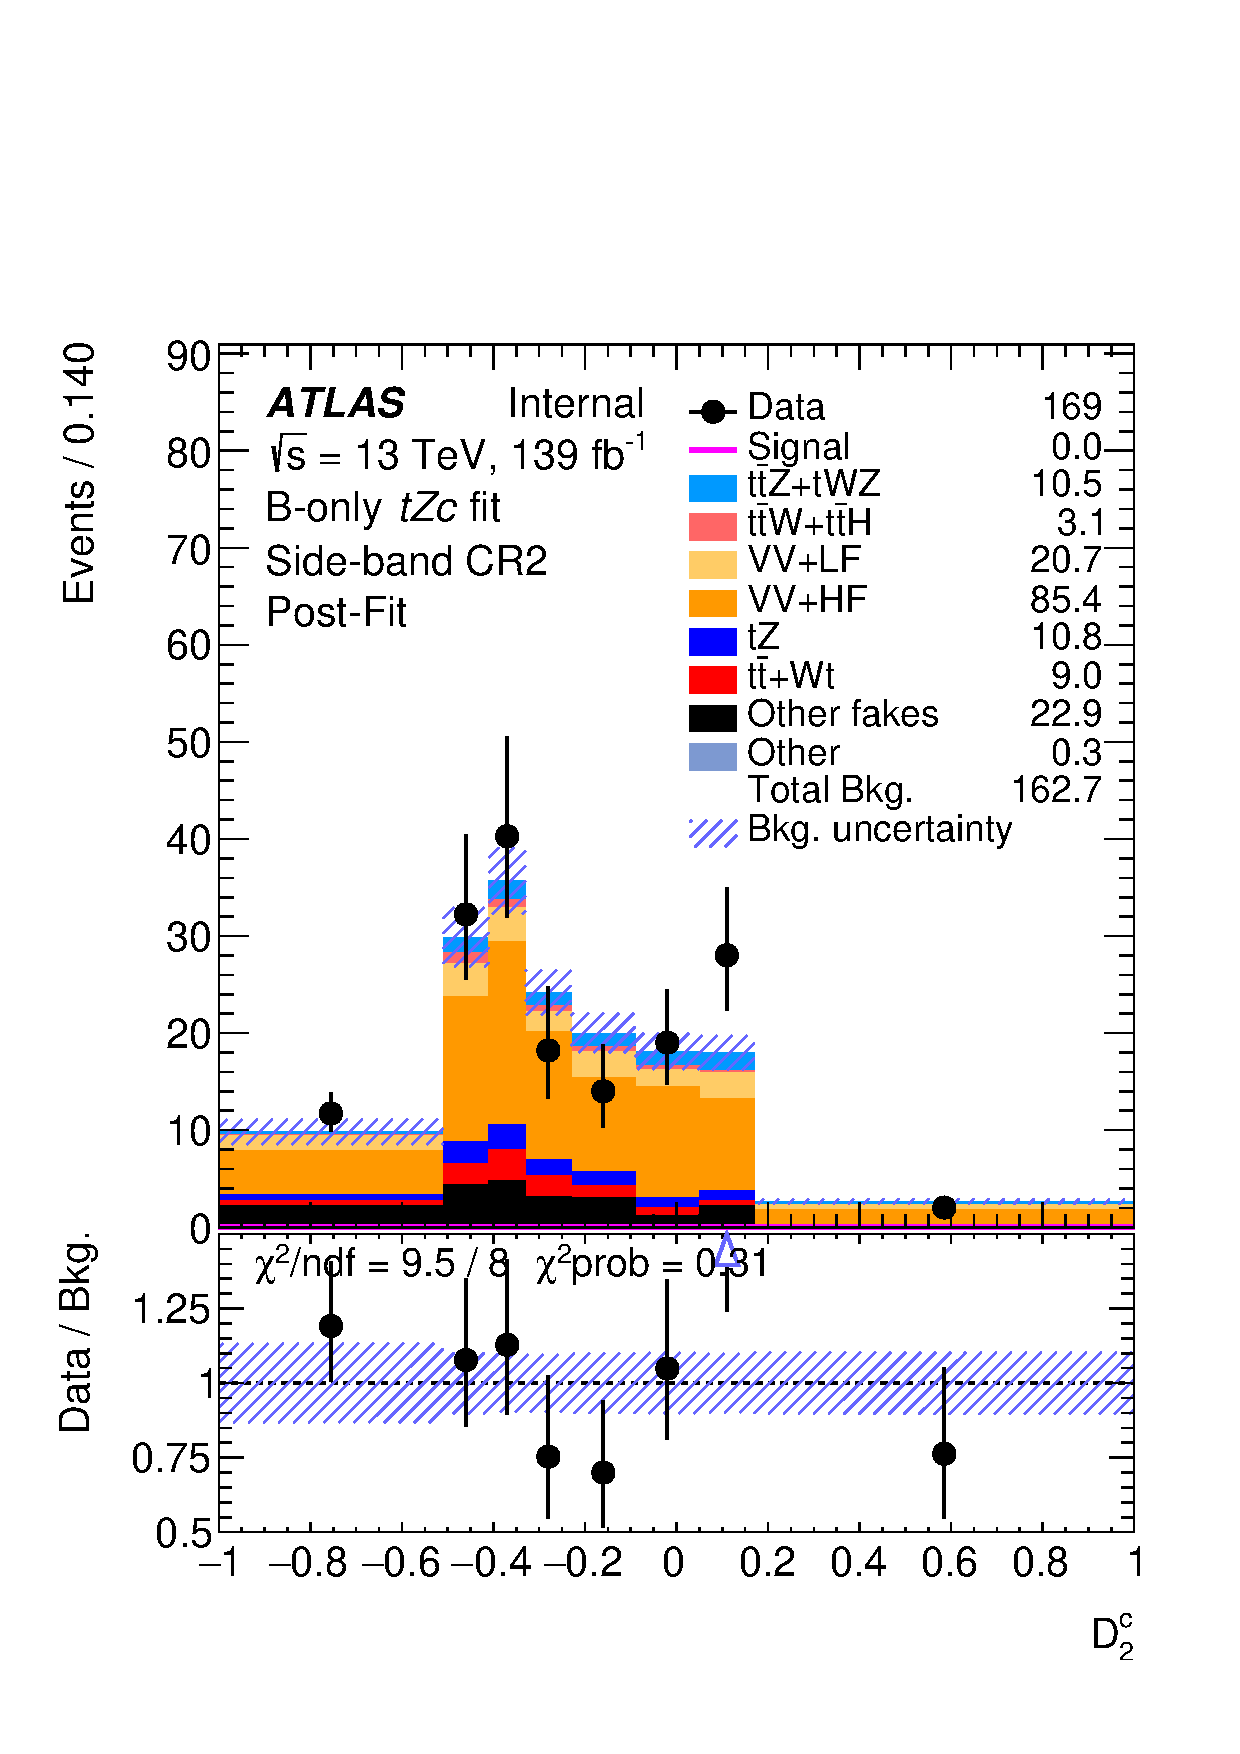
\includegraphics[width=.45\textwidth]{Appendices/AP9/figures/BONLY_CRSR_DL1rc_unblind/Plots/SBCR2_postFit} \\
	\end{tabular}
	\caption{Pre-fit (left) and post-fit (right) BDTG output distributions in the side-band CRs for the B-only \tZc fit in SRs+CRs with data.
		\ErrStatSys
	}%
	\label{fig:stat:tzc:bonly:crsr:crplots:1_unb}
\end{figure}

\begin{figure}[htbp]
	\centering
	\begin{tabular}{cc}
		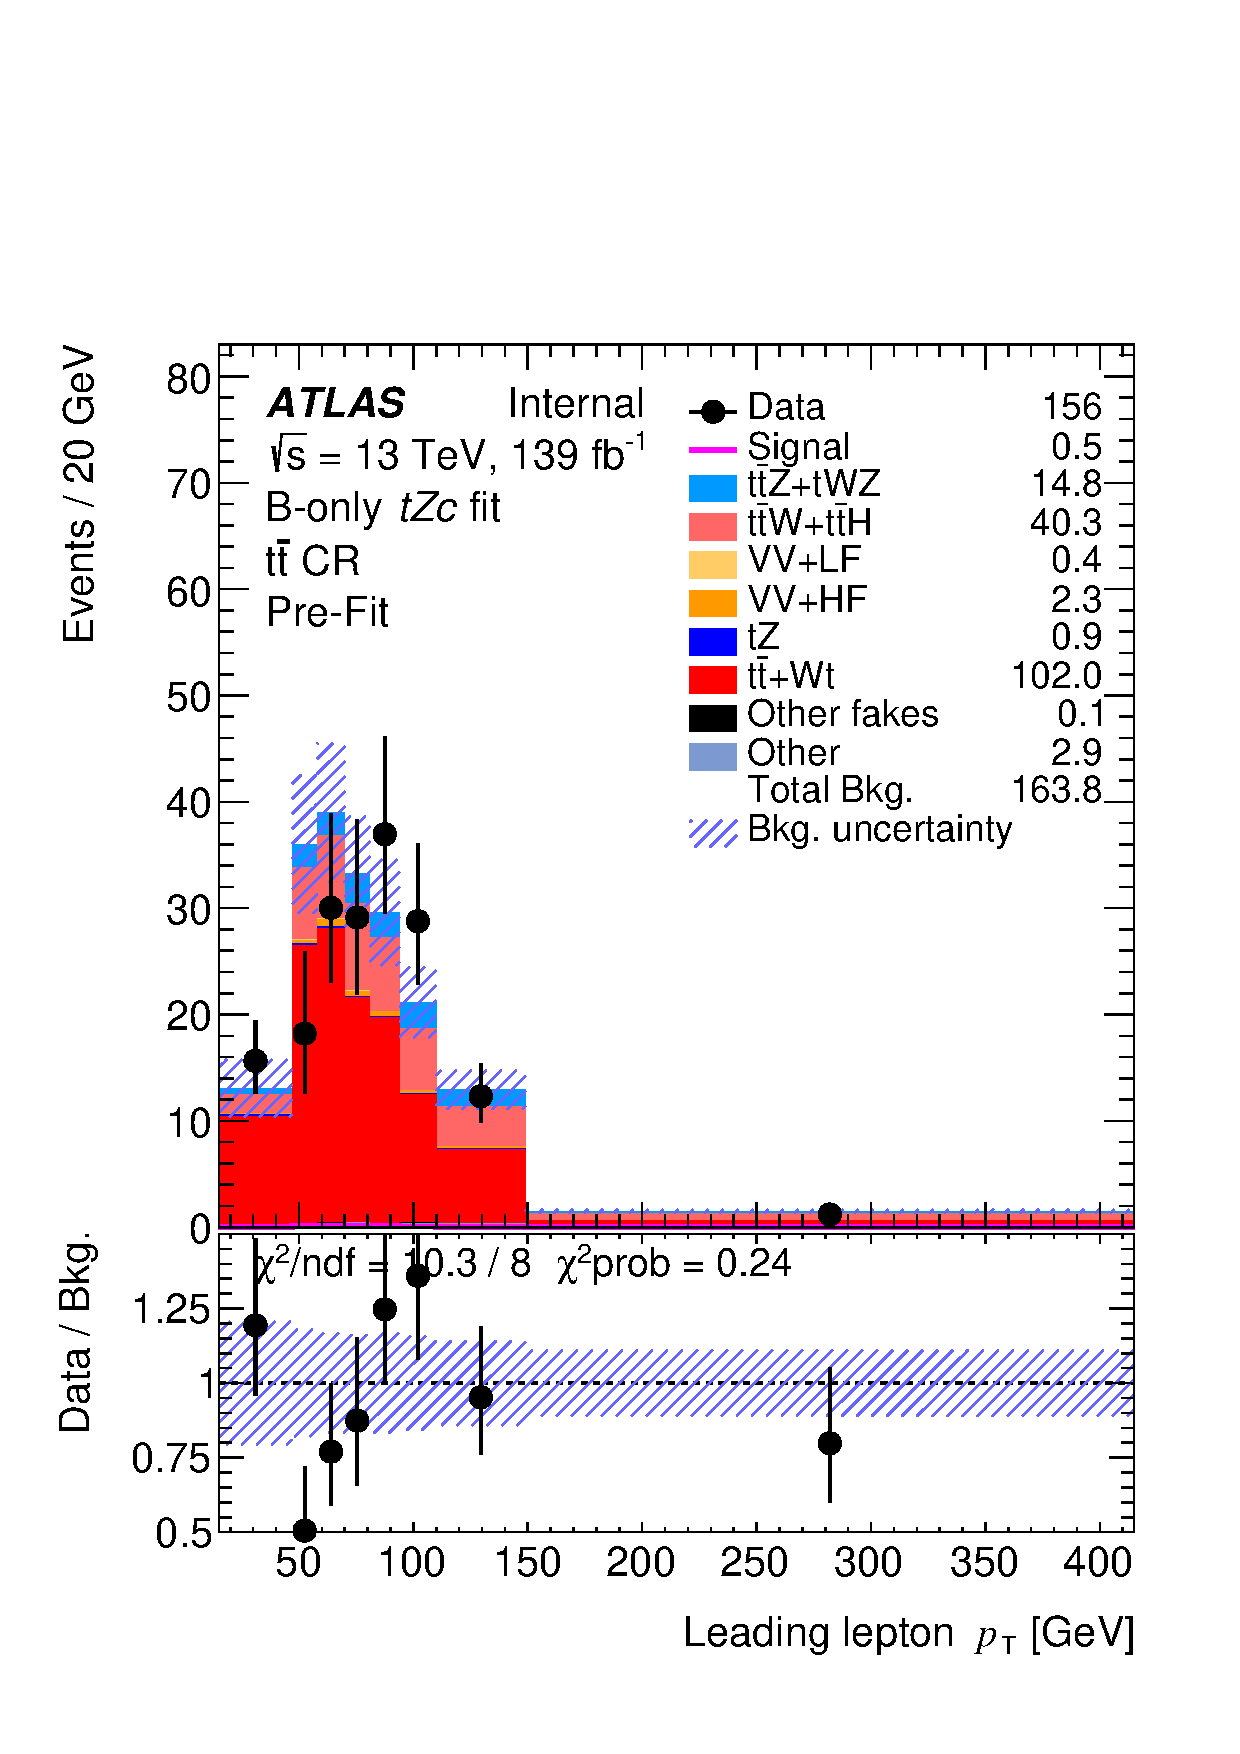
\includegraphics[width=.45\textwidth]{Appendices/AP9/figures/BONLY_CRSR_DL1rc_unblind/Plots/TTCR} &
		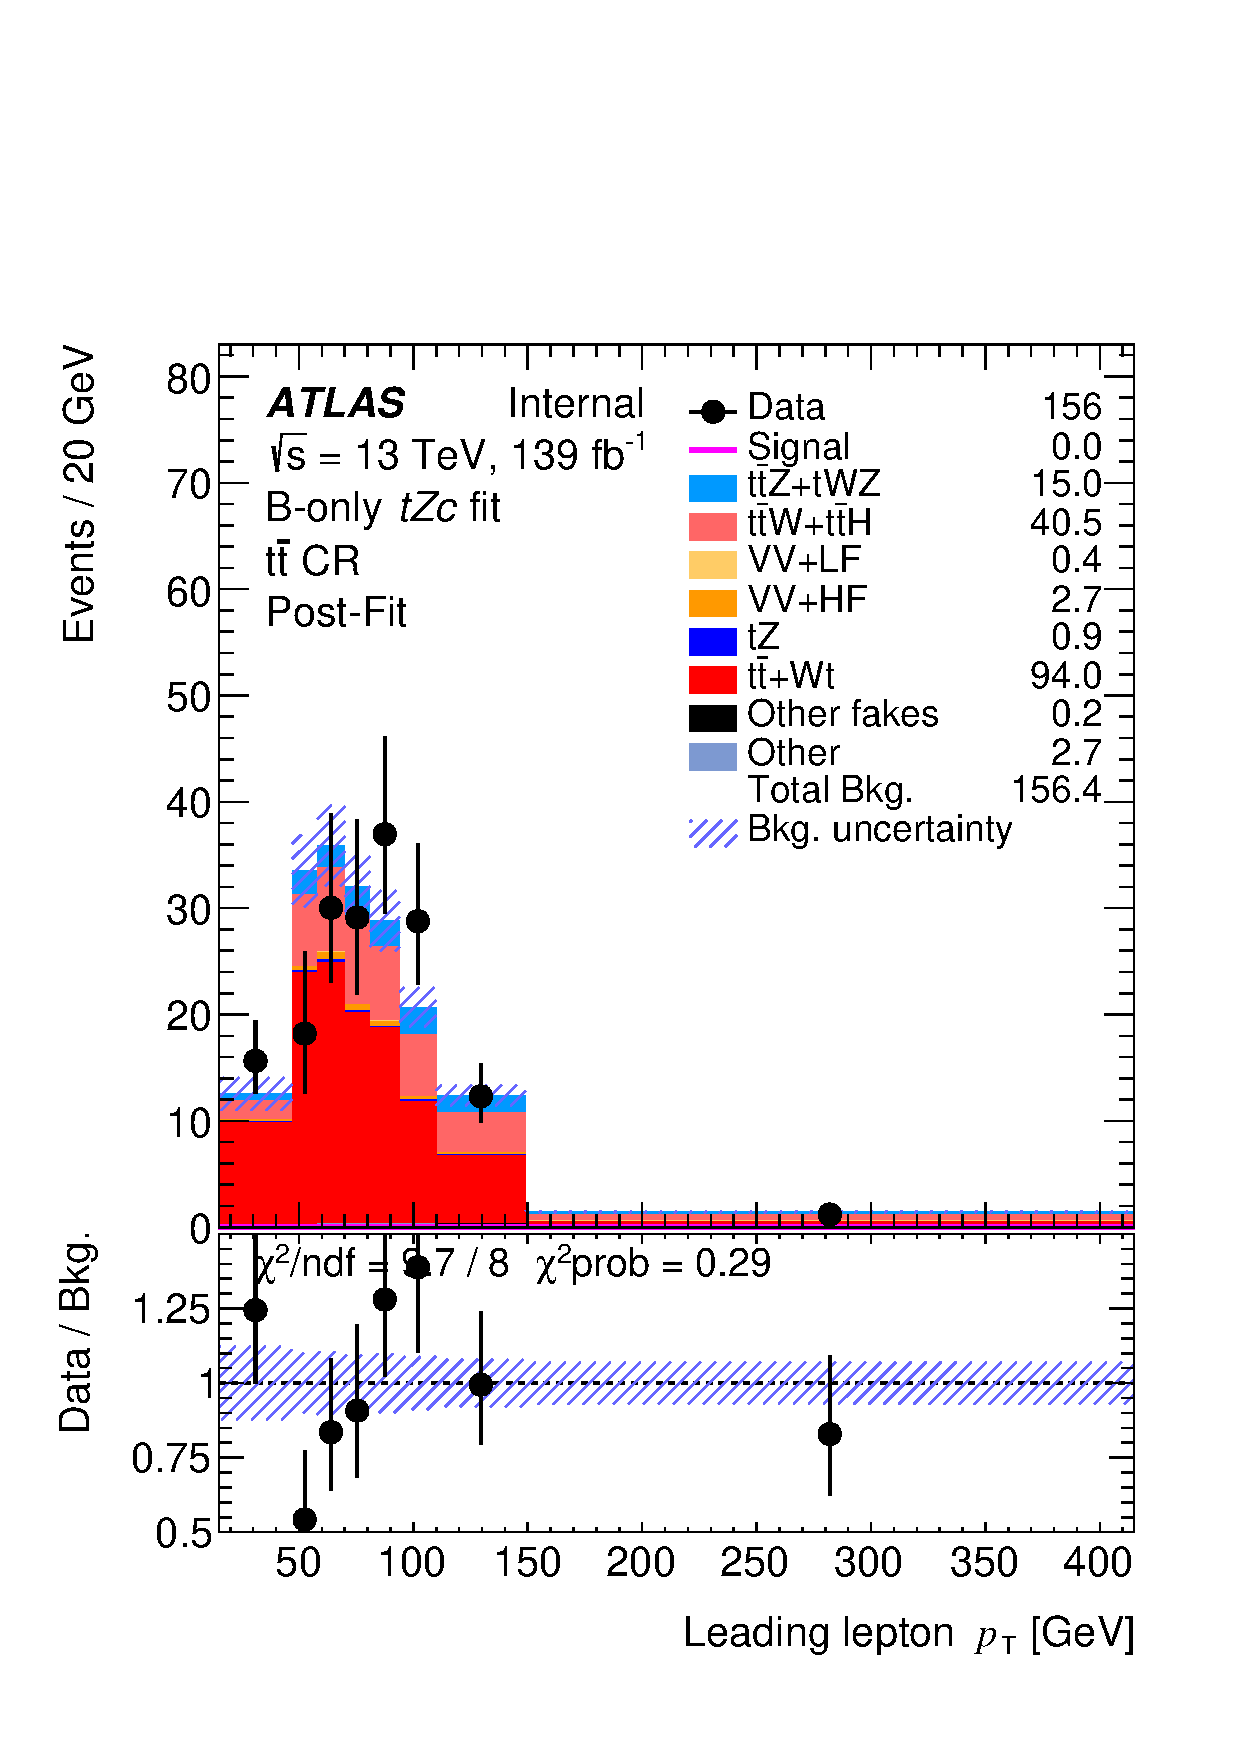
\includegraphics[width=.45\textwidth]{Appendices/AP9/figures/BONLY_CRSR_DL1rc_unblind/Plots/TTCR_postFit} \\
		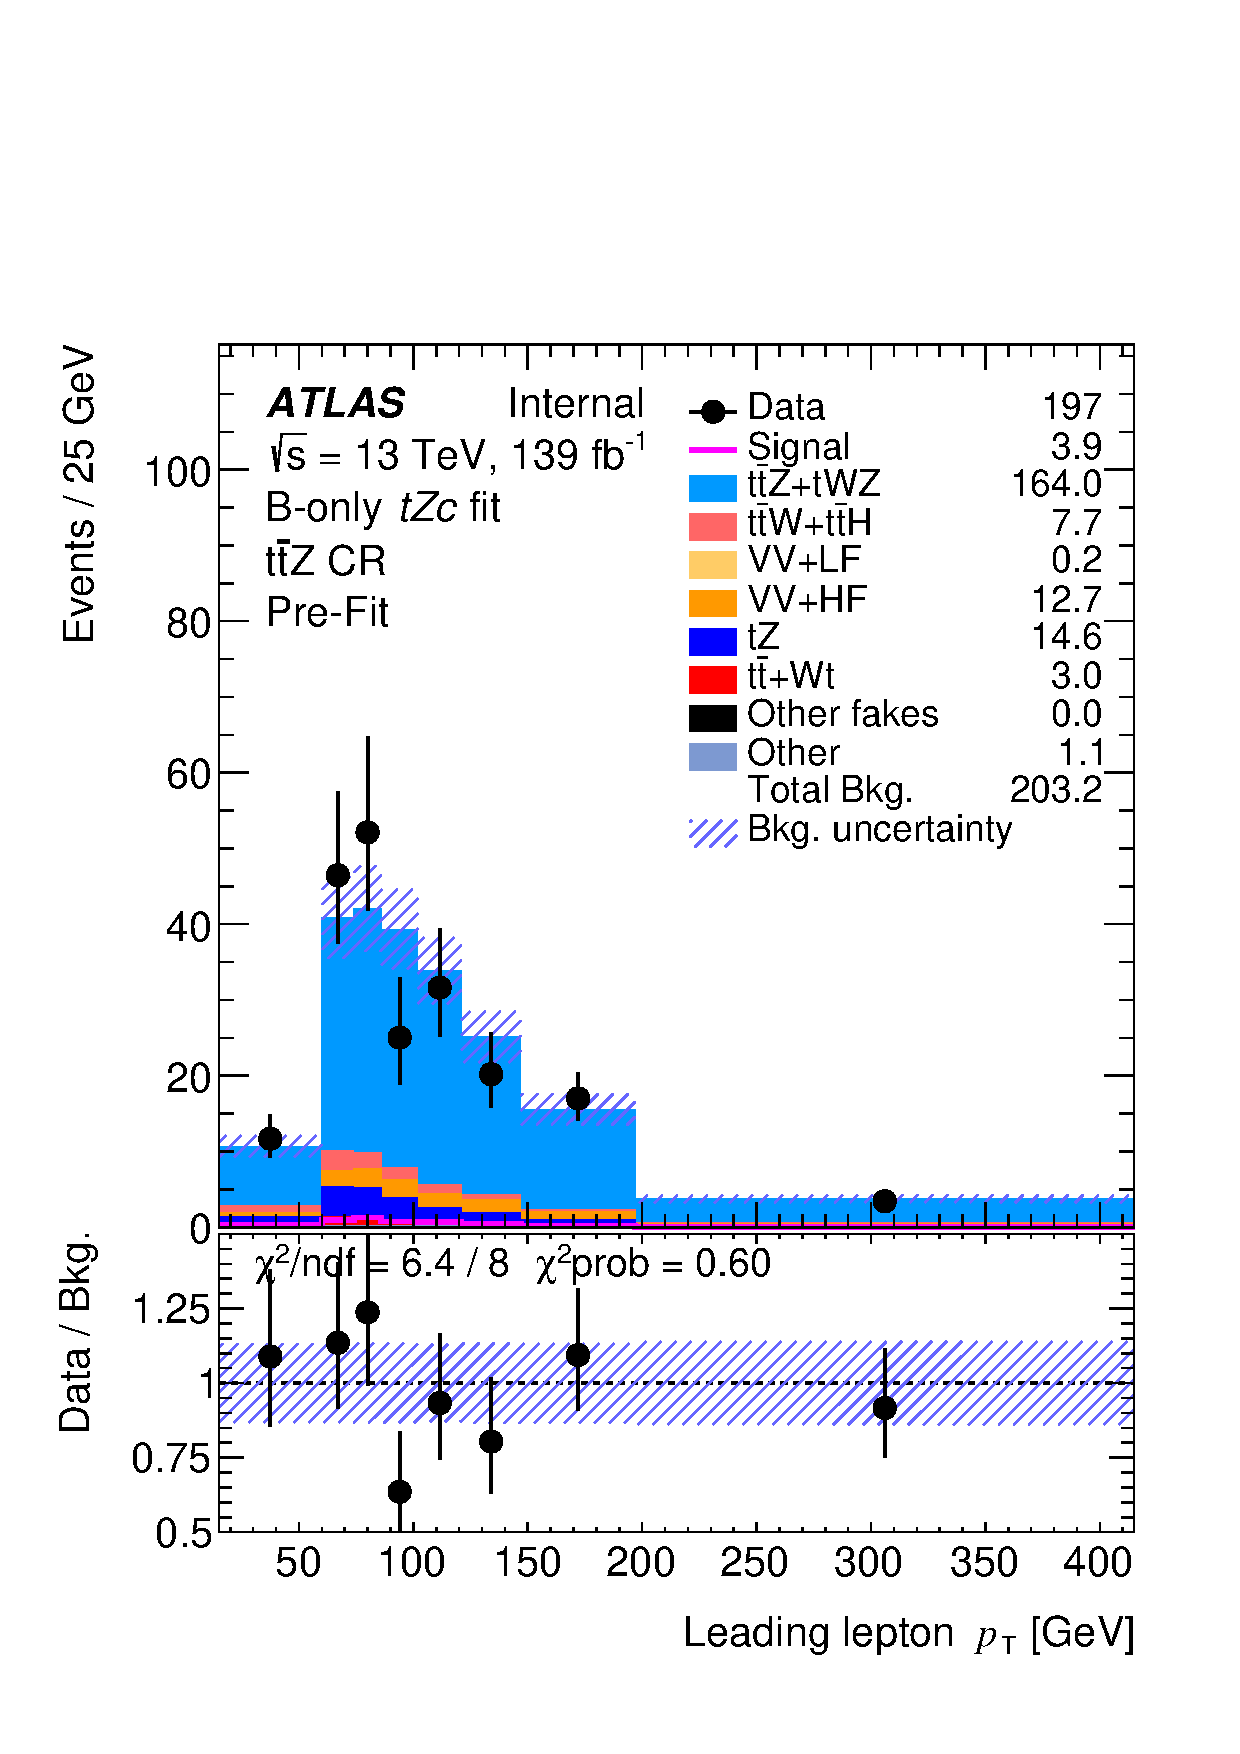
\includegraphics[width=.45\textwidth]{Appendices/AP9/figures/BONLY_CRSR_DL1rc_unblind/Plots/TTZCR} &
		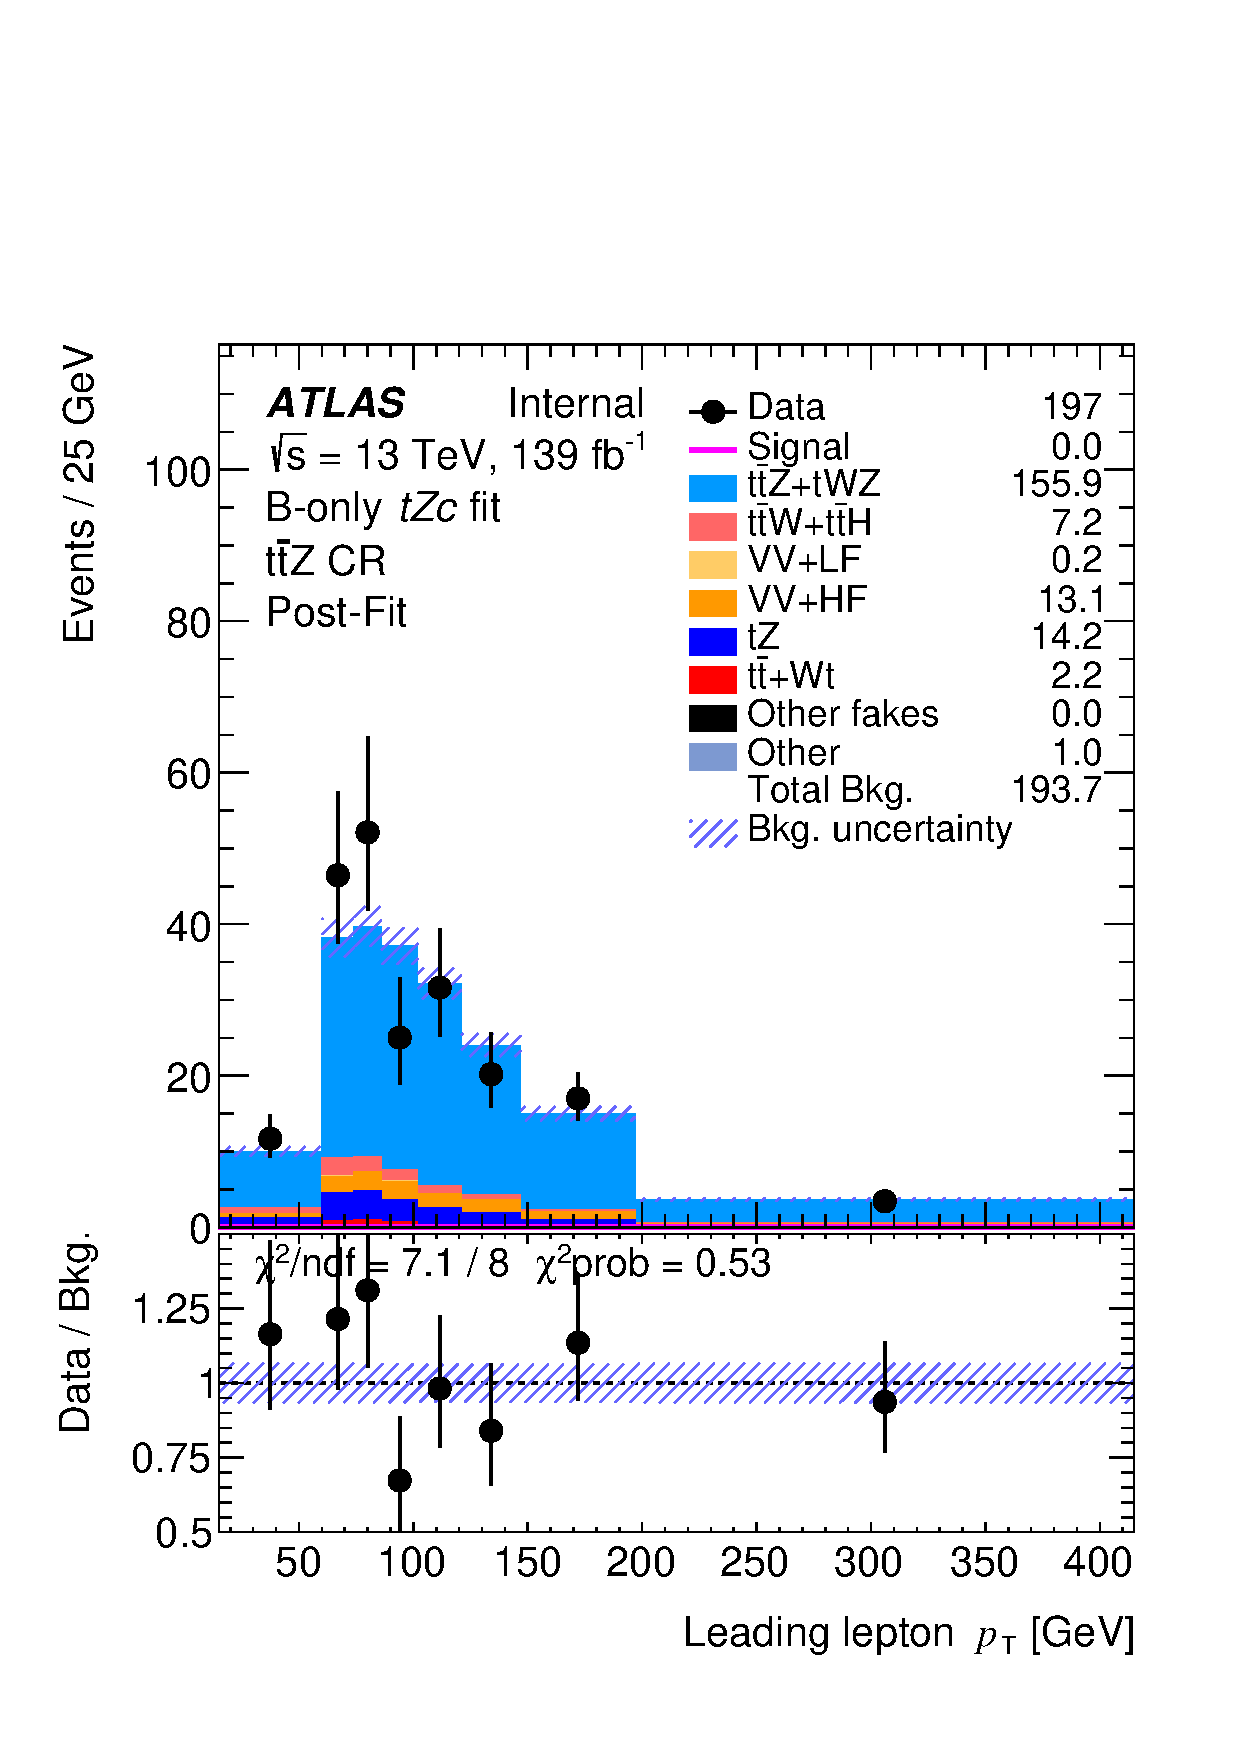
\includegraphics[width=.45\textwidth]{Appendices/AP9/figures/BONLY_CRSR_DL1rc_unblind/Plots/TTZCR_postFit} \\
	\end{tabular}
	\caption{Pre-fit (left) and post-fit (right) leading lepton \pt distributions in the \ttbar and \ttZ CRs for the B-only \tZc fit in SRs+CRs with data.
		\ErrStatSys
	}%
	\label{fig:stat:tzc:bonly:crsr:crplots:2_unb}
\end{figure}

\FloatBarrier
\clearpage
\noindent From the likelihood fit under the Background-only hypothesis no evidence for the FCNC $\mathrm{\Pqt\rightarrow\PZ\Pqc}$ signal is found but a good agreement between data and Standard Model is observed.
In the absence of signal, the 95\% CL upper limit is set on $\mathrm{BR (\Pqt\rightarrow\PZ\Pqc)}$.\\
\Cref{fig:stat:tzc:bonly:crsr:CLsPlot} shows the observed and expected $\mathrm{CL_{s}}$ as a function of $\mathrm{BR (\Pqt\rightarrow\PZ\Pqc)}$.\\
The observed limit is $\mathrm{BR (\Pqt\rightarrow\PZ\Pqc)}<11.8\times 10^{-5}$, inside the $\pm$1$\sigma$ band of the expected limit: $\mathrm{BR (\Pqt\rightarrow\PZ\Pqc)}<9.5\times 10^{-5}$.
\begin{figure}[htbp]
	\centering
	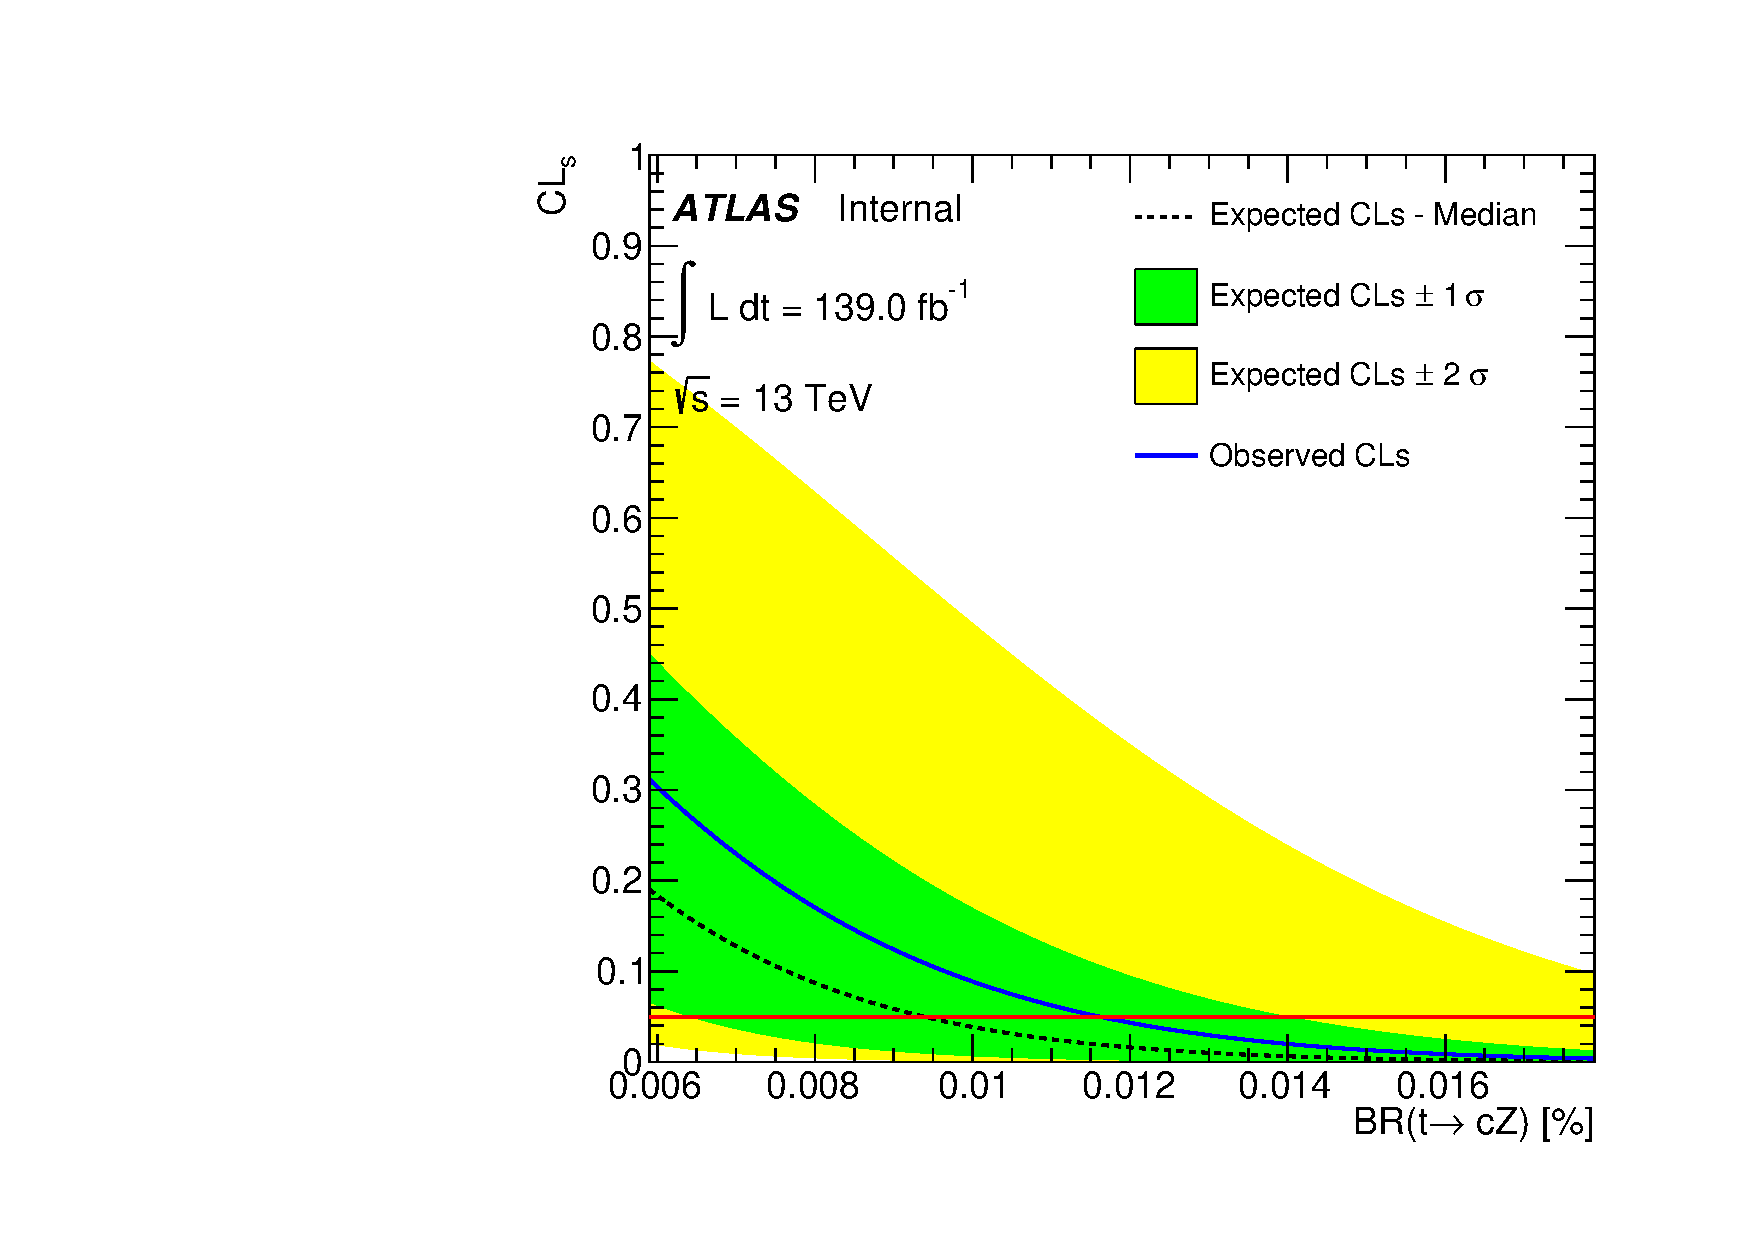
\includegraphics[width=.6\textwidth]{Appendices/AP9/figures/BONLY_CRSR_DL1rc_unblind/CLsPlot}
	\caption{$\mathrm{CL_{s}}$ vs $\mathrm{BR (\Pqt\rightarrow\PZ\Pqc)}$ plot. The median expected $\mathrm{CL_{s}}$ under the Background-only hypothesis
		(black dashed line) is displayed along with the $\pm$1 and $\pm$2 standard deviations bands
		(green and yellow, respectively). The solid red line at $\mathrm{CL_{s}= 0.05}$ denotes the threshold below
		which the hypothesis is excluded at 95\% CL.}
	\label{fig:stat:tzc:bonly:crsr:CLsPlot}
\end{figure}

\begin{table}[htbp]
	\centering
	\begin{tabular}{lc} 
		\toprule
		& BR ($\Pqt\rightarrow\PZ\Pqc) [\times 10^{-5}]$  \\
		\midrule
		Observed  				   					& 11.8  \\
		Expected -1$\sigma$   				  &   6.9 \\
		Expected                    				&  9.5 \\
		Expected +1$\sigma$  				 &  13.8 \\		
		\bottomrule
	\end{tabular}
	\caption{
		Observed and expected 95\% CL upper limits on the FCNC $\Pqt\rightarrow\PZ\Pqc$ branching ratio. 
		The expected central value is shown together with the $\pm$1$\sigma$ bands.
	}%
	\label{tab:results:limits}
\end{table}

